% LaTeX-Vorlage Version 3.1,  Juli 2011
% erstellt von Dr. Andreas Drauschke (andreas.drauschke@technikum-wien.at) und Dr. Susanne Teschl (susanne.teschl@technikum-wien.at)
% geringf"ugig adaptiert von Harald Stockinger (harald.stockinger@technikum-wien.at)

 
\documentclass[a4paper,bibtotoc,oneside]{scrbook} 
% F"ur kurze Arbeiten w"are auch die Dokumentklasse "scrartcl" ausreichend. In diesem Fall ist "section" die h"ochste Ebene ("chapter" gibt es dann nicht).
% \documentclass[a4paper,bibtotoc,oneside]{scrartcl}


% verlinkte Querverweise im pdf
\usepackage{hyperref}

% deutsche Anpassungen
%\usepackage[ansinew]{inputenc}
\usepackage[utf8]{inputenc}
\usepackage[T1]{fontenc}
\usepackage[ngerman]{babel}




% mathematische Symbole
\usepackage{amsmath,amssymb,amsfonts,amstext}

% Kopfzeilen frei gestaltbar
\usepackage{fancyhdr}
\lfoot[\fancyplain{}{}]{\fancyplain{}{}}
\rfoot[\fancyplain{}{}]{\fancyplain{}{}}
\cfoot[\fancyplain{}{\footnotesize\thepage}]{\fancyplain{}{\footnotesize\thepage}}
\lhead[\fancyplain{}{\footnotesize\nouppercase\leftmark}]{\fancyplain{}{}}
\chead{}
\rhead[\fancyplain{}{}]{\fancyplain{}{\footnotesize\nouppercase\sc\leftmark}} 

% Farben im Dokument m"oglich
\usepackage{color}

% Schriftart Helvetica
\usepackage{helvet}
\renewcommand{\familydefault}{cmss} 

% Graphiken einbinden: hier f"ur pdflatex
\usepackage[pdftex]{graphicx}

\usepackage{array}

\usepackage{subfigure} 

\usepackage{multirow}

% H"ohe und Breite des Textk"orpers etwas gr"osser definieren
\setlength{\textheight}{225mm}
\setlength{\textwidth}{1.05\textwidth}

% weniger Warnungen wegen "uberf"ullter Boxen
\tolerance = 9999
\sloppy

% Anpassung einiger "Uberschriften 
\renewcommand\figurename{Abbildung}
\renewcommand\tablename{Tabelle}



\begin{document}

% Kopf- und Fusszeilen initiieren
\pagestyle{fancy}

% Deckblatt:
\thispagestyle{empty}
\begin{picture}(0,0)
\color{white}\sffamily
\put(-101,-749){
\includegraphics[width=1.002\paperwidth, height=\paperheight]{img/BM_2011.pdf}}
\put(220,-670){
\includegraphics[width=0.5\textwidth]{img/FHTW_Logo_4c.pdf}}
\put(-30, -20){\bfseries\huge MASTER THESIS}
\put(-30,-50){\Large zur Erlangung des akademischen Grades}
\put(-30,-70){\Large \glqq Master of Science in Engineering\grqq}
% Titel des Studienganges einf"ugen:
\put(-30,-90){\Large im Studiengang Industrielle Elektronik}
% Titel der Arbeit einf"ugen:
% Die Minipage wird gesetzt, damit auch mehrzeilige Titel m"oglich werden.
\put(-32,-180){
\begin{minipage}{14cm}
\bfseries\huge Aufbau eines automatisierten Mess- und Auswertesystems zur Bestimmung der Bestrahlungsst"arkeverteilung in einem station"aren Sonnensimulator
\end{minipage}
}
% Name der Autorin/des Autors eingeben:
\put(-30,-270){\large Ausgef"uhrt von: Thomas Schmatz BSc}
% Personenkennzeichen der Autorin/des Autors eingeben:
\put(-30,-290){\large Personenkennzeichen: 1010300002}
% Name der Begutachterinnen/der Begutachter eingeben:
\put(-30,-330){\large 1. BegutachterIn: DI Bernhard Kubicek}
\put(-30,-350){\large 2. BegutachterIn: DI (FH) Thomas Krametz }
\put(-30,-390){\large Wien, \today} % das Datum des letzten Kompilierens wird automatisch eingesetzt
\color{black}
\end{picture}

\newpage


\section*{Eidesstattliche Erkl"arung}\thispagestyle{empty}
\glqq Ich erkl"are hiermit an Eides statt, dass ich die vorliegende Arbeit selbst"andig angefertigt habe. 
Die aus fremden Quellen direkt oder indirekt "ubernommenen Gedanken sind als solche kenntlich gemacht. 
Die Arbeit wurde bisher weder in gleicher noch in "ahnlicher Form einer anderen Prüfungsbehörde vorgelegt
und auch noch nicht ver"offentlicht. Ich versichere, dass die abgegebene Version jener im Uploadtool entspricht.\grqq\\[5\baselineskip]
\rule{5cm}{0.2pt}\hfill\rule{5cm}{0.2pt}\\
\phantom{Datum }Ort, Datum\hfill Unterschrift\hspace{15mm}

\newpage



\section*{Kurzfassung}\thispagestyle{empty}
Die Arbeit umfasst die Planung und Realisierung eines selbstfahrenden Messroboters, der die Bestrahlungsst"arkeverteilung in der Prüfebene eines station"aren Sonnensimulators erfasst. Neben den Einstrahlungsdaten werden werden zus"atzliche Informationen über die Umgebungsbedingungen im Prüfkanal aufgezeichnet. Bei der Umsetzung wurden Rapid-Prototyping Techniken (3D-Druck, Platinenfr"ase und Lasercutter) eingesetzt. Behandelt werden theoretische Grundlagen und normative Anforderungen an station"are Sonnensimulatoren, sowie Messunsicherheitsberechnungen und Validierung des Gesamtsystems.
\\ \vfill
% Bitte 3-5 deutsche Schlagw"orter eingeben, die die Arbeit charakterisieren:
\paragraph*{Schlagw"orter:} Schlagwort 1, Schlagwort 2, Schlagwort 3, Schlagwort 4, Schlagwort 5


\newpage

\section*{Abstract}\thispagestyle{empty}
Text Text Text Text Text Text Text Text Text Text Text Text Text Text Text Text Text Text Text Text Text Text Text Text ...
\\ \vfill
% Bitte 3-5 englische Keywords eingeben, die die Arbeit charakterisieren:
\paragraph*{Keywords:} Keyword 1, Keyword 2, Keyword 3, Keyword 4, Keyword 5
\newpage

\section*{Danksagung}\thispagestyle{empty}
Ich danke meinen Eltern für die Unterstützung und Geduld, die sie w"ahrend des Studiums aufgebracht haben.
Ich danke meinen Hochschulbetreuer für die umfangreiche Betreuung.
Ich danke meinen Firmenbetreuer Thomas Krametz für die Zeit die er sich genommen hat.
... (Rohfassung!!!!)
\newpage

\tableofcontents\thispagestyle{empty}
\newpage

\setcounter{page}{1}

% Falls die Kapitel"uberschriften zu lang f"ur die Kopfzeile oder das Inhaltsverzeichnis sind, so erzielt man
% dort Kurzformen der Kapitelbezeichnungen mittels:
% \chapter[Kurzform]{Lange "Uberschrift}
\chapter{Aufgabenstellung}
\section{Warum Module im Sonnensimulator} \thispagestyle{empty}
Ein Sonnensimulator simuliert die Wirkung von Sonnenlicht auf Prüfobjekte. Für die Prüfung von PV-Modulen ersetzt ein stationärer Sonnensimulator das natürliche Sonnenlicht, das ist notwendig weil aufgrund von Jahreszeit und Witterung nicht immer 1000W pro Quadratmeter mit den AM1,5 Spektrum zur Verfügung stehen.
Es bedarf der Erklärung einiger wichtiger Begriffe. AM steht für Air Mass, die Lufthülle der Erde, die zum einem das leben auf diesen Planeten ermöglicht, zum anderen muss das Sonnenlicht die Erdatmosphäre durchdringen. Dabei wird das Licht abgeschwächt und die spektrale Zusammensetzung verändert, weil bestimmte Moleküle (O2, H2O, CO2) der Luft einige Wellenlängenbereiche sehr gut absorbieren. 
 

\begin{figure}[htbp]
\centering
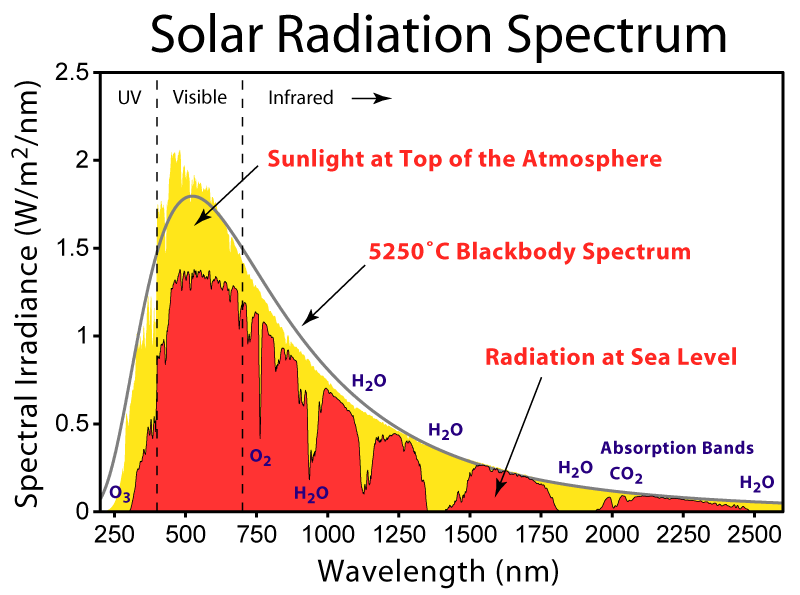
\includegraphics[width=75mm]{img/Solar_Spectrum.png}
\caption{Spektrum der Sonne}\label{sunspec}
\end{figure}


\section{Sonnensimulator Aufbau}\thispagestyle{empty}
10 Lampen zu je 4 kW. Angeordnet in 2 Reihen zu je 5 Lampen. Die Lampen sind höhenverstellbar.
Die Leistung der Lampen lässt sich einzeln ansteuern.
Die Testobjekte, z.B. ganze Module oder auch einzelne Zellen liegen in einer Lade.
Die Prüfebene ist 2,50 mal 4 Meter groß. Nur ein teil dieser Ebene wird verwendet.
Die Prüfebene liegt innerhalb eines Windkanales, der oben für die Strahlung durchsichtig ist.
Der Windkanal verengt sich, damit die Windgeschwindigkeit ansteigt, um eine konstante Kühlleistung wegen der sich erwärmenden Luft zu haben. 

\begin{figure}[htbp]
\centering
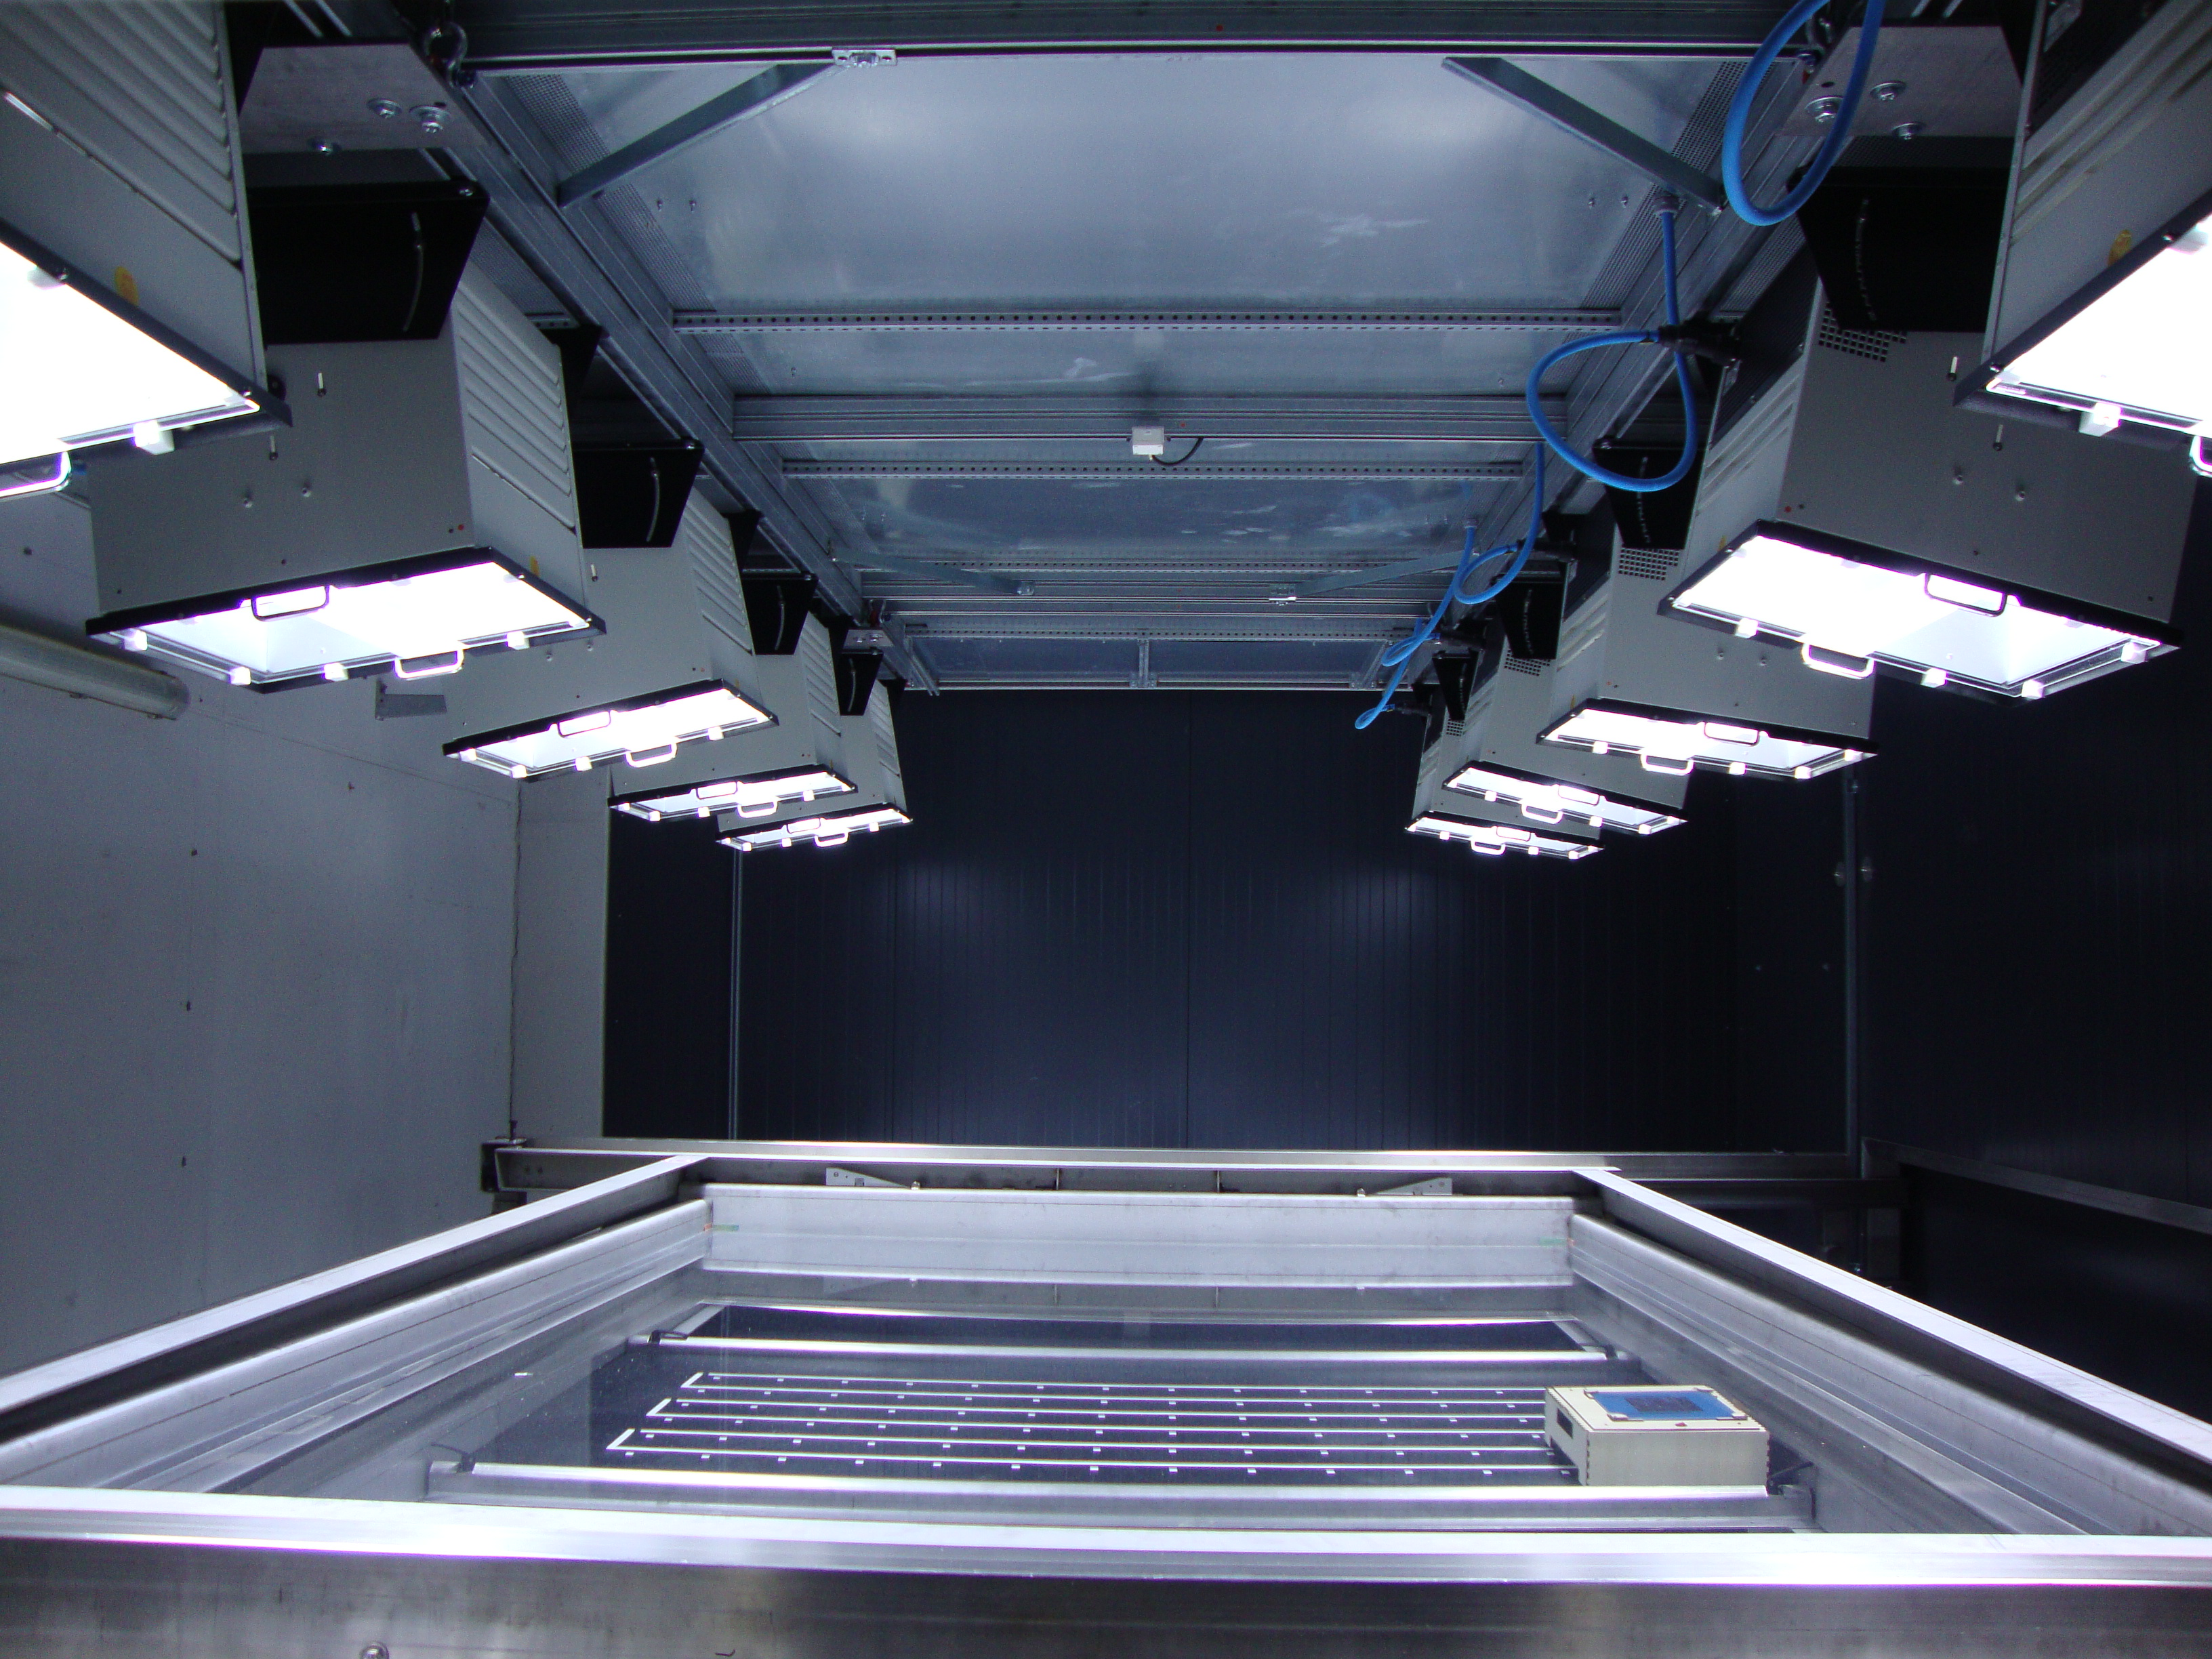
\includegraphics[width=75mm]{img/sunsimulator.jpg}
\caption[Sonnensimulator]{Sonnensimulator}\label{sunsim}
\end{figure}


\section{Normative Anforderungen an den Sonnensimulator}\thispagestyle{empty}
Akkreditierung,Begründnung warum Messroboter, Alte Ergebnisse, Alte Messmethode

In IEC 60904-9 legt die Anforderungen an Sonnensimulatoren fest.

\begin{figure}[htbp]
\centering
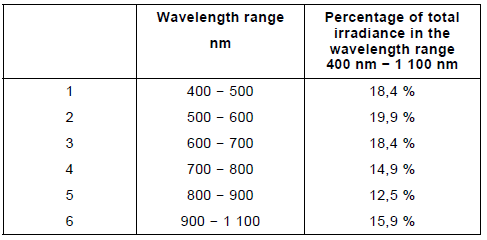
\includegraphics[width=75mm]{img/spectral.png}
\caption[Spektralle Strahlungsverteilung]{Spektralle Strahlungsverteilung nach IEC 60904-9}\label{sectral}
\end{figure}

\begin{figure}[htbp]
\centering
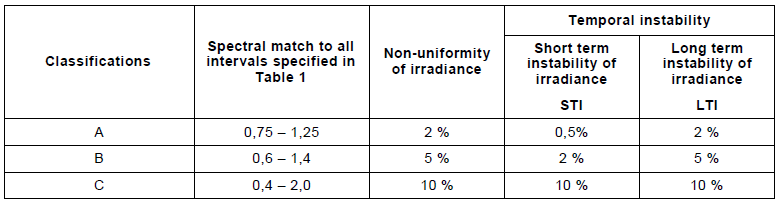
\includegraphics[width=75mm]{img/simclass.png}
\caption[Simulatorklassen]{Simulatorklassen}\label{Sim2}
\end{figure}



\section{Theorie Referenzzelle}\thispagestyle{empty}
Es gibt verschiedene Solarzelltechnologien. Wirtschaftlich bedeutend sind im Moment nur kristalline Siliziumzellen und Dünnschichtzellen. Die kristallinen Siliziumzellen werden in monokristalline Zellen und polykristalline Zellen unterschieden. Beide zusammen amchen über 80\% des weltweiten Photovoltaikmarktes aus. Als Referenzzelle für Messungen werden ausschließlich kristalline Zellen verwendet. Wichtig ist, dass die Referenzzelle eine ähnliche spektralle Empfindlichkeit hat wie die zu messenden Zelle bzw. das zu messende Modul.
Siliziumsolarzellen bestehen aus einer großflächigen Diode. Die Sperrschicht ist dabei dem Sonnenlicht ausgesetzt. Gelangt ein Lichtquanten in die Sperrschicht kann aufgrund des inneren Photoeffektes ein Elektron/Loch Paar erzeugt werden. Durch das elektrische Feld in der Sperrschicht werden die Ladungsträger getrennt bevor sie kombinieren können. Elektronen bewegen aufgrund ihrer negativen Ladung entgegen der Feldrichtung in die n-Zone. Löcher wandern in Feldrichtung zur raumladungsfreien p-Zone. Die Leerlaufspannung einer Solarzelle ist kleiner als die Diffusionsspannung.
\begin{figure}[htbp]
\centering
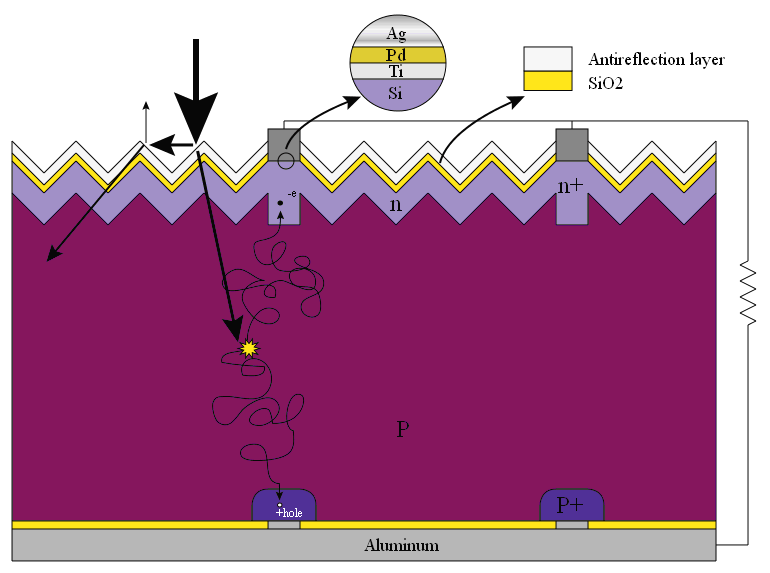
\includegraphics[width=125mm]{img/cell.png}
\caption{Schematischer Aufbau einer Solarzelle}\label{cell}
\end{figure}


Die unbeleuchtete Solarzelle ist funktioniert wie eine normale Halbleiterdiode, die einen Durchlassstrom von p- nach n-Seite fließen lässt, falls eine Spannung von p nach n anliegt. Bei Beleuchtung wird zusätzlich ein Photostrom erzeugt, welcher proportional zur Bestrahlungsstärke und der Zellfläche ist. Das Ersatzschaltbild~\ref{esb} besteht daher aus einer Stromquelle, dazu parallel einer Diode, einen Parallelwiderstand und einem Serienwiderstand. Der Parallelwiderstand fasst Kurzschlüsse zusammen, die realen Solarzellen am Rand oder an den Korngrenzen auftreten können. Mit dem Serienwiderstand werden alle Spannungsabfälle in der Solarzelle erfasst. Eine ideale Solarzelle hat einen Serienwiderstand von null und einen Parallelwiderstand von unendlich. 
\begin{figure}[htbp]
\centering
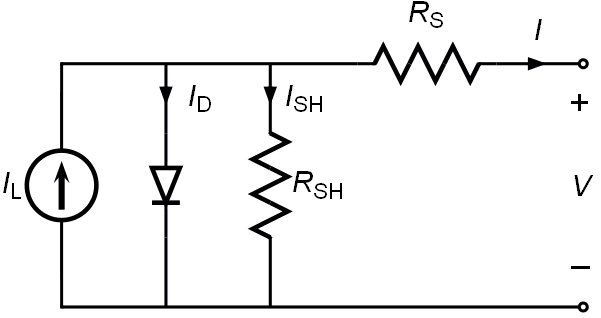
\includegraphics[width=100mm]{img/esb.png}
\caption{Ersatzschaltbild}\label{esb}
\end{figure}

Durch den zusätzlichen Photostrom verschiebt~\ref{kennlinie} sich die Diodenkennline. Bei Leerlaufspannung bzw. Kurzschlussstrom gibt die Solarzelle keine Leistung ab. Der Punkt der Kennlinie mit der maximalen Leistung wird als Maximum Power Point (MPP) bezeichnet.

Der Füllfaktor berechnet sich aus Strom im maximalen Leistungspunkt $I_{mp}$, Spannung am maximalen Leistungspunkt $U_{mp}$, Kurzschlusstrom $I_{sc}$ und Leerlaufspannung $U_{oc}$.
  \begin{equation}
     FF = \frac {I_{mp} U_{mp}} {I_{sc} U_{oc}}
  \end{equation}
  
Die Leerlaufspannung hängt von der Temperatur ab. Mit steigender Temperatur wird der Bandabstand kleiner. Dadurch können Photonen kleinerer Energie absorbiert werden und somit steigt der Kurschlussstrom. Die Leistung im MP-Punkt sinkt mit steigender Temperatur.
Zusammenhang von Kurzschlusstrom und Leerlaufspannung.
  \begin{equation}
     I_{sc} = I_0 ( e^{\frac {q U_{oc}}{k T}} - 1 )
  \end{equation}
  Hierbei ist $I_{0}$ der Söttigungsstrom der Diode (im Ersatzschalbild ~\ref{esb}):
    \begin{equation}
     I_{0} = A ( \frac { q D_{e} n_i^2} {L_e N_A} + \frac {q D_h n_i^2} {L_h N_D})
  \end{equation}
  
  $N_A$ und $N_D$ sind die Dichten von Akzeptoren sowie Donatoren, $D_e$ und $D_h$ sind die Diffusionskoeffizienten von Elektronen und Löchern, $n_i$ ist die intrinsische Ladungsträgerdichte, $L_e$ und $L_h$ sind Diffusionslängen von Elektronen und Löchern. Alles materialabhängige Konstanten.
  
  \begin{equation}
     U_{sc} = \frac {k T}{q} ln (\frac {I_L}{I_0} + 1 )
  \end{equation}
  
  Hier ist $I_L$ der Photostrom, und berechnet sich :
  
  \begin{equation}
     I_{L} = q A G ( L_e + W + L_h )
  \end{equation}
Bei $A$ handelt es sich um die Zellfläche, bei $G$ um die Generationsrate von Elektron-Löcher-Paaren und bei $W$ um die W um die Breite der Raumladungszone. 

\begin{figure}[htbp]
\centering
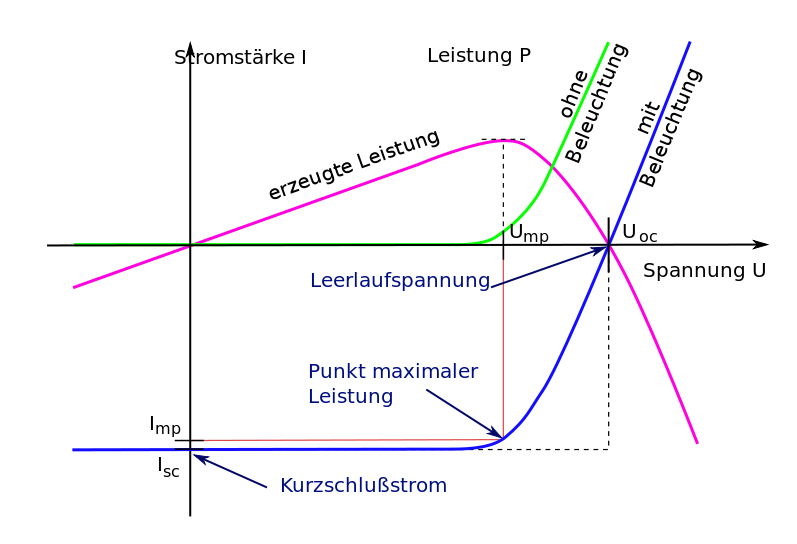
\includegraphics[width=125mm]{img/kennlinie.png}
\caption{Dunkel- und Hellkennlinien}\label{kennlinie}
\end{figure}

\begin{figure}[htbp]
\centering
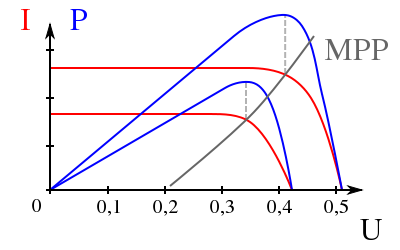
\includegraphics[width=75mm]{img/mpp.png}
\caption{Abhängigkeit des MPP von der Einstrahlung}\label{mpp}
\end{figure}





\chapter{Entwicklungprozess}\thispagestyle{empty}

\section{Hardwaredesign}\thispagestyle{empty}
\subsection{Mecanum-Platform}\thispagestyle{empty}
Das Mecanum-Rad ist ein Rad, das Fahrman"over in jede Richtung erlaubt, ohne dass das Fahrzeug mit einer mechnischen Lenkung ausgestattet ist. Bennnt ist es nach dem schwedischen Unternehmen Macanum AB in welchen dieses Rad 1971 entwickelt wurde. 
Erreicht wird die Wendigkeit der Fahrzeuge durch den Einsatz von Mecanum R"adern, die einzeln angetrieben werden. Diese R"ader bestehen aus einer Felge, auf der unter einem Winkel von 45 Grad lose, ballige Rollen so angebracht sind, dass sie "uber den Abrollumfang wieder einen exakten Kreis bilden.
Durch die Schr"aganordnung der Rollen entstehen beim Antreiben des Rades 2 Kraftkomponenten. Gegeneinander gerichtete Kr"afte der einzelnen Räder werden über die Achsen und den Rahmen kompensiert. Die übrigen Kräfte addieren sich zur resultierenden Fahrtrichtung. Auf diese Weise sind durch entsprechendes Ansteuern der einzelnen Räder omnidirektionale Fahrmanöver möglich, ohne dass das Fahrzeug mit einer mechanischen Lenkung ausgestattet ist. 
\begin{figure}[htbp]
\centering
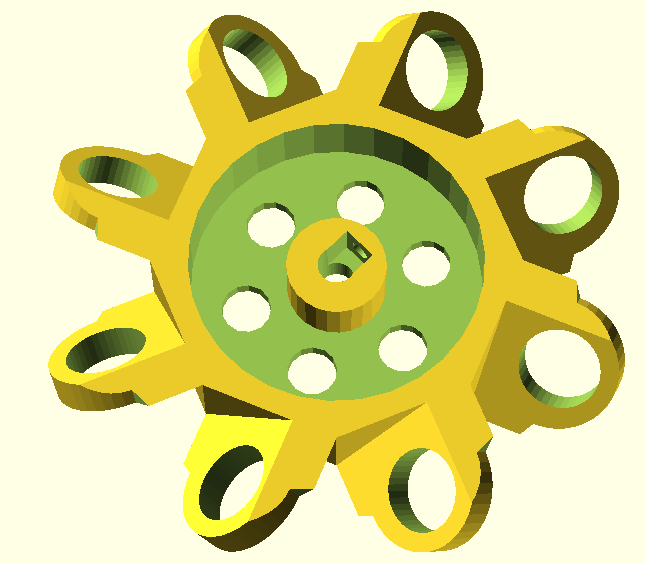
\includegraphics[width=75mm]{img/wheel.png}
\caption{Die Felge des Mecanum Rades}\label{rad}
\end{figure}

\begin{figure}[htbp]
\centering
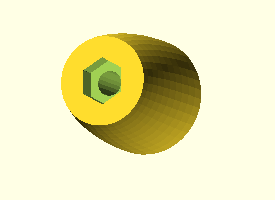
\includegraphics[width=75mm]{img/roller.png}
\caption{Eine der 16 Rollen pro Reifen}\label{rolle}
\end{figure}

\begin{figure}[htbp]
\centering
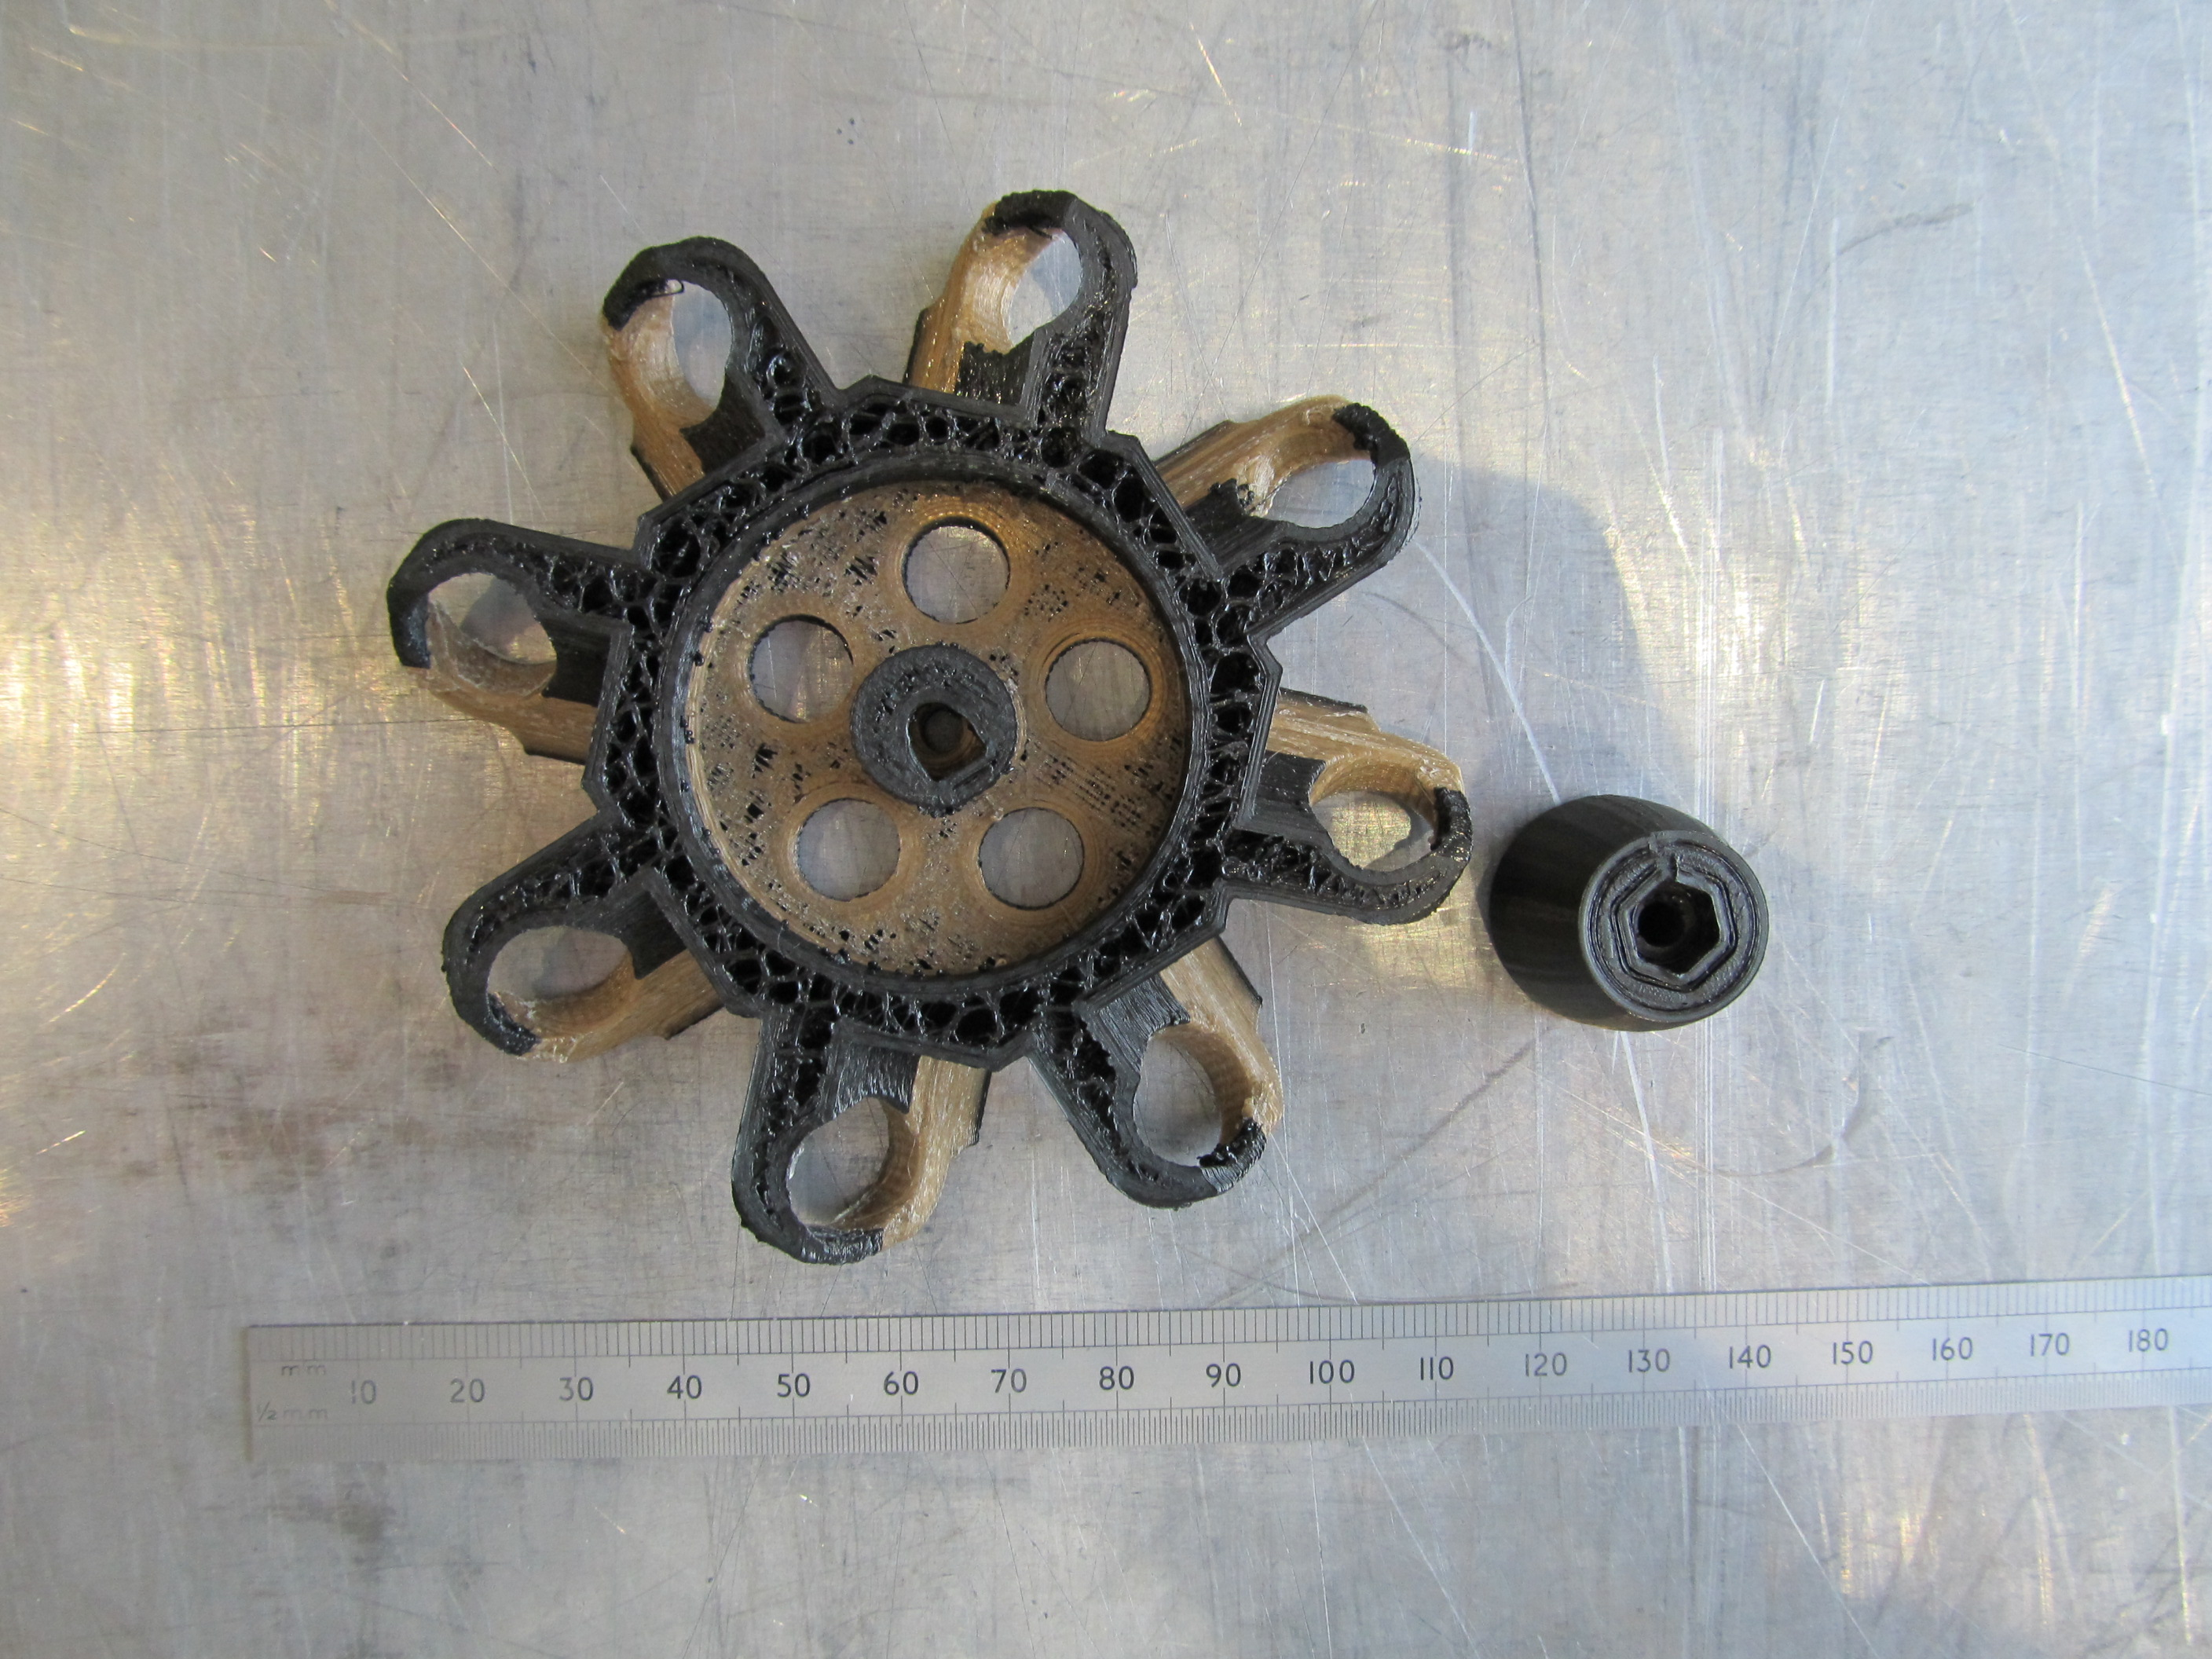
\includegraphics[width=75mm]{img/roller_wheel.jpg}
\caption{Ein gedrucktes Rad samt Rolle}\label{rollerad}
\end{figure}

\subsection{Chassis}\thispagestyle{empty}

\noindent Die Chassis wurde aus Sperrholz gefertigt. Dieses Holz wurde gewählt weil es leicht zu bearbeiten, robust und UV-beständig ist. Das Design dafür entstand mit QCAD. QCAD ist ein 2-dimensionales CAD Programm. 
Die Größe der Chassis wurde bestimmt durch: \begin{itemize}
\item Den Durchmesser und der Breite der Mecanum Räder, die Räder liegen innerhalb der Chasis, damit die Räder vor der UV Strahlung geschützt sind, und die Räder keinen Einfluss (Beschattung oder Reflexionen) auf die Messzelle haben.
\item Die Größe der Motoren.
\item Der Arduino , die Motorsteuerelektronik und die Messelektronik
\item Der Akku zur Stromversorgung, die dazugehörende Akku Spannungsüberwachung und der Ein/Aus Schalter.
\item Die Abmessung der Messzelle.
 \end{itemize}

\noindent Die Einzelteile wurden mit einem Lasercutter aus einer großen Sperrholzplatte geschnitten. Die Einzelteile wurden teilweise miteinander verleimt damit eine zukünftige Wartung problemlos möglich ist, wurde der Aufbau verschraubt ausgeführt.
Die Motoren sind verschraubt, damit ein Austausch möglich ist. Einzelne Räder als auch die Rollen lassen sich bei Bedarf austauschen.
Das Chassis besteht aus 3 Teilen: \begin{itemize}
\item Der Bodenplatte
\item Die Seitenwände
\item Das Dach mit der Aufnahme für die Messzelle
\end{itemize}

\begin{figure}[htbp]
\centering
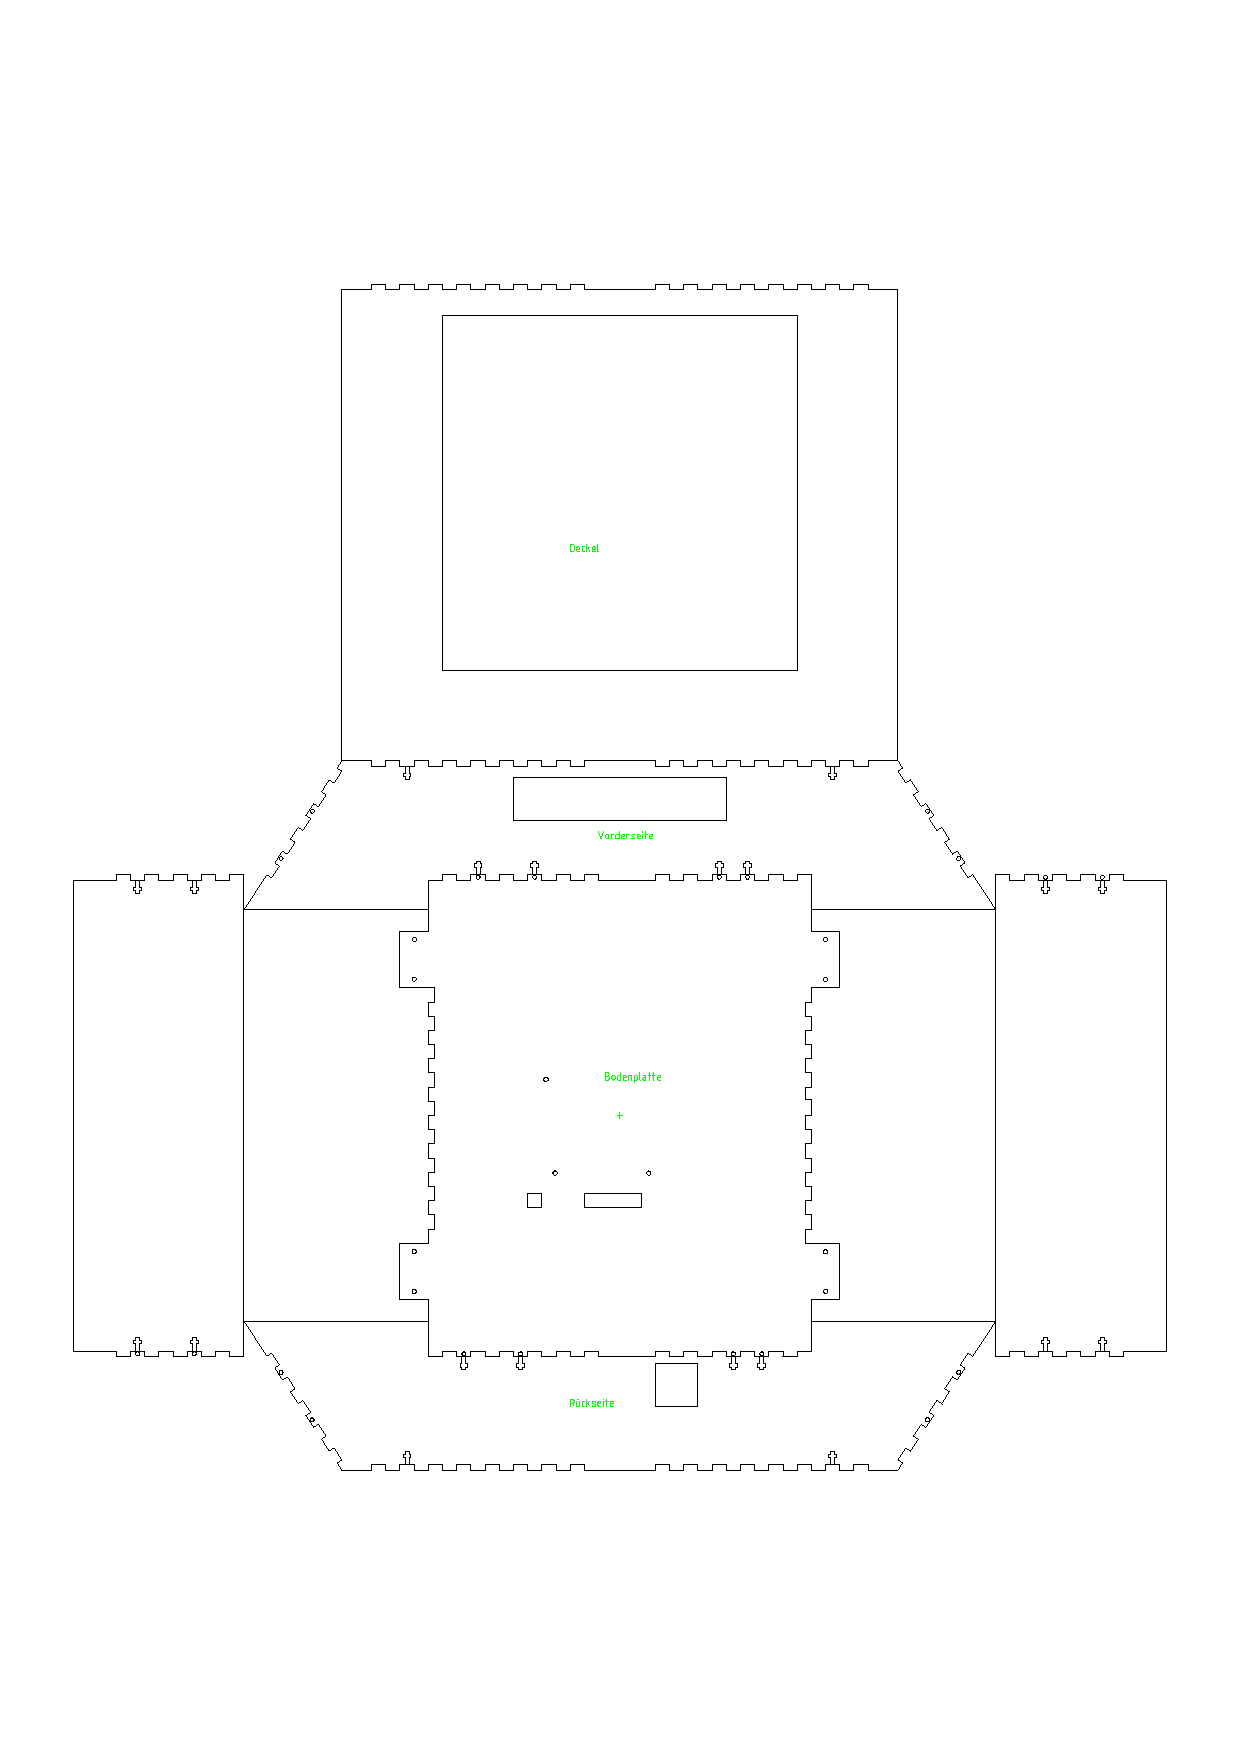
\includegraphics[width=125mm]{img/gehause.pdf}
\caption[Chassis]{Chassis}\label{chassis}
\end{figure}


\section{Steuerungselektronik}\thispagestyle{empty}

Dieser Abschnitt beschreibt die Entwicklung der Elektronik. Die Funktionalität wurde auf verschiedene Module aufgeteilt. Das erleichtert die Platzierung der Elektronik innerhalb des Messroboters, und den Austausch von Komponenten im Fehlerfall. 
Das Gehirn des Roboters ist ein Arduino Mega 2560 Mikrocontroller Board. Darauf aufgesteckt ist ein sogenanntes Shield, eine selbst entwickelte Platine, das die $\pm$5V Spannungsversorgung, die Schnittstellen zu den anderen Platinen und einen SD-Karten Einschub beheimatet.
Es gibt 3 Messplatinen, eine für den Kurzschlussstrom der Messzelle, zwei für Temperaturmessungen. Eine Platine überwacht den Ladezustand des Akkus. Die Motorensteuerung ist auf einer eigenen Paltine beheimatet.
 
\subsection{Motorensteuerung}\thispagestyle{empty}


Eine H-Brücke~\ref{hbridge} erlaubt es einem Gleichstrommotor sich in zwei Richtungen zu drehen. Dafür müssen immer zwei schräg gegenüber liegende Schalter eingeschaltet sein. Zum Beisiel die Schalter S1 und S4 für die Drehrichtung im Uhrzeigersinn, S2 und S3 für die Drehrichtung gegen den Uhrzeigersinn. Zwei untereinander liegende Schalter dürfen nicht gleichzeitig eingeschaltet werden. Es muss einen hardwaretechnischen Schutz gegen diese art von Kurzschlüssen geben. Ein softwaretechnischer Schutz reichte dem Autor nicht, nachdem ein früher Prototyp der Motortreiberdplatine sich in Rauch aufgelöst hatte. Deshalb wurde für den Roboter eine integrierte H-Brücke (NJM2670) verwendet, mit einer logischen Verriegelung, die keinen Kurzschluss produzieren kann. 
\newline
Die Drehzahl bei konstanter Versorgungsspannung lässt sich mit Pulsweitenmodulation variieren.

\begin{figure}[htbp]
\centering
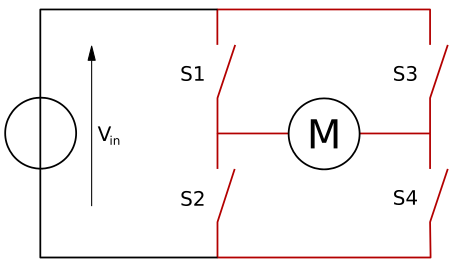
\includegraphics[width=75mm]{img/hbridge.png}
\caption[H-Brücke]{H-Brücke}\label{hbridge}
\end{figure}

Die Gleichspannungsmotoren sind Getriebemotoren mit der Bezeichnung RB 35, und einem Übersetzungsverhältnis von 1:200. Die maximale Versorgungsspannung wurde mit 12V angegeben. Die Drehzahl beträgt bei 12V Versorgungsspannung 20 Umdrehungen pro Minute.
Der Roboter wird mit einem Lithium-Ionen-Akku versorgt. Die Spannung beträgt, abhängig vom Ladezustand zwischen 16,4V und 15,0V. Damit es zu keiner Überlastung der 12V-Motoren, kommt wurde bei der Pulsweitenmodulation ein maximales Tastverhältnis von 50\% eingehalten.

\begin{figure}[htbp]
\centering
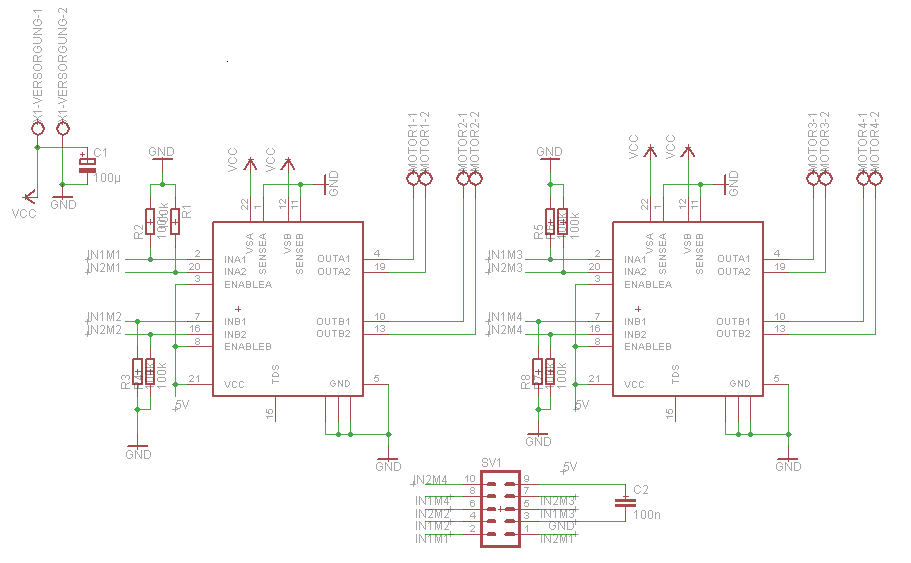
\includegraphics[width=150mm]{img/HBrucke.png}
\caption[H-Brücke Schaltung]{H-Brücke Schaltung}\label{hbridge2}
\end{figure}


\subsection{Optische Sensorik}\thispagestyle{empty}
Der Roboter ist ein Linienfolge. Damit er einer Linie folgen kann, muss diese zuerst zuverl"assig erkannt werden. 
Als Sensor wurde ein CNY70 verwendet. Der CNY 70 ist ein Reflexionsensor. Der Sensor wird in einem fixen Abstand zu einer Ebene montiert. Eine LED sendet Licht mit 950nm aus, welches an der Ebene reflektiert wird. Damit können Unterschiede des Reflektionkoeffizienten, umgangssprachlich der Farbe, gemessen werden. Die Anordung 9 solcher Sensoren in einem 3 mal 3 Array kann sowohl vertikale als auch horizontale Linien erkennen, sowie Ecken.

\begin{figure}[htbp]
\centering
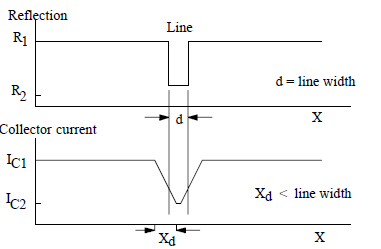
\includegraphics[width=75mm]{img/cny70.png}
\caption{Der Strom durch den Phototransistor ist abhängig von der Reflektiviät des Untergrundes}\label{cny1}
\end{figure}

\begin{figure}[htbp]
\centering
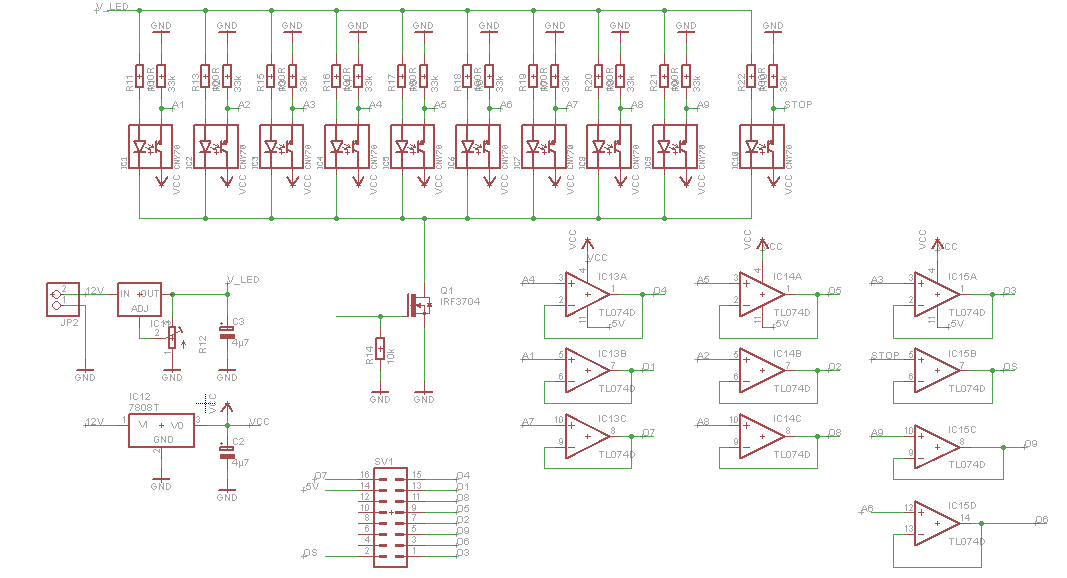
\includegraphics[width=125mm]{img/array.png}
\caption{Der Schaltplan des Sensorarrays}\label{array}
\end{figure}

\begin{figure}[htbp]
\centering
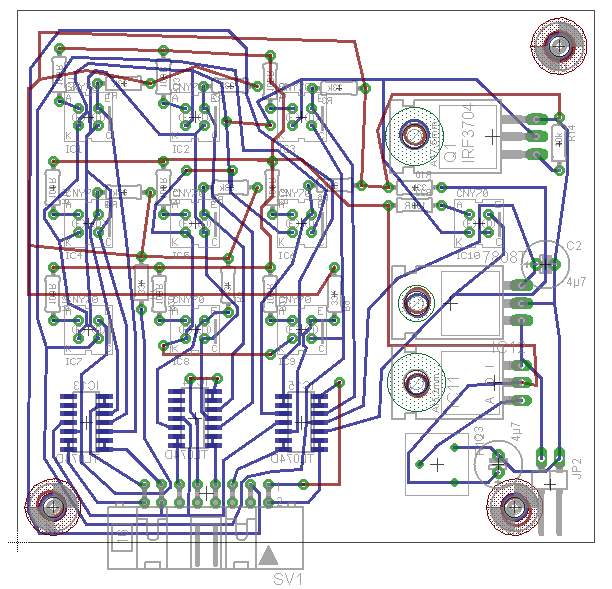
\includegraphics[width=125mm]{img/array2.png}
\caption{Das Layout des Senorarrays}\label{array2}
\end{figure}


\begin{figure}[htbp]
\centering
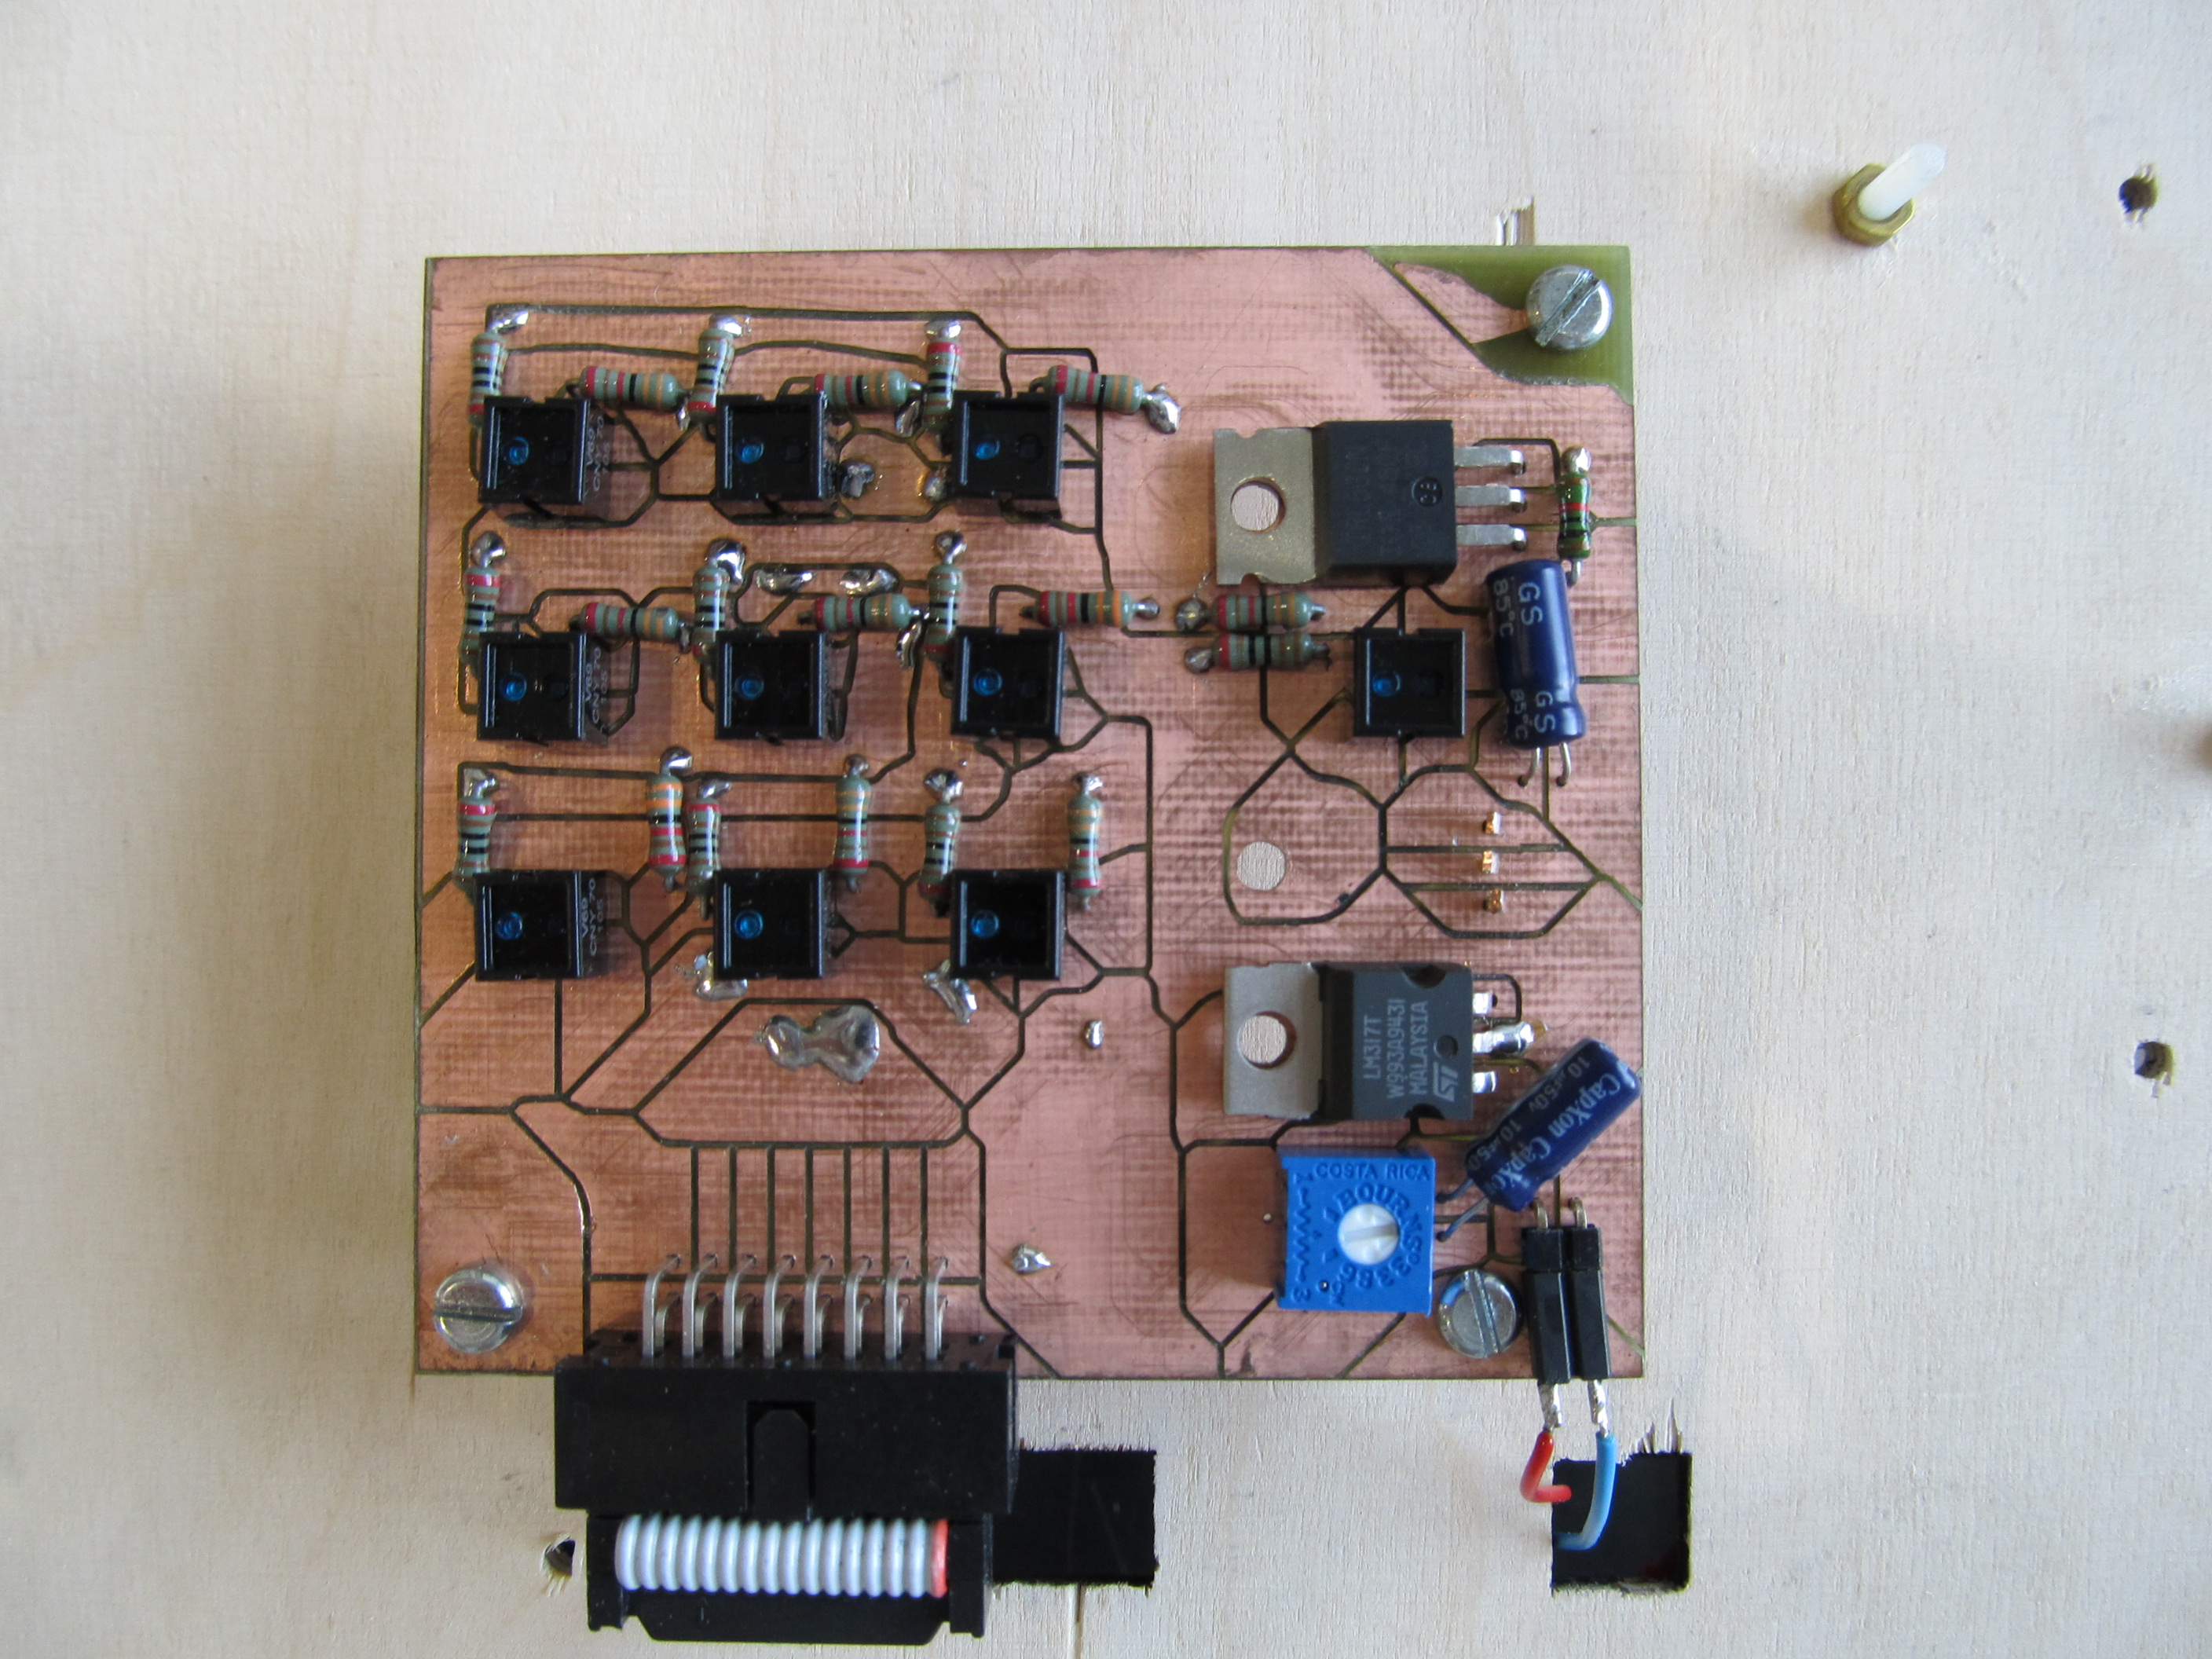
\includegraphics[width=125mm]{img/sensor_array.jpg}
\caption{Das unter dem Roboter montierte Sensorarrayt}\label{array3}
\end{figure}



\subsection{Spannungversorgung}\thispagestyle{empty}
Aku-handling, "Uberwachung der Akkuspannung, Alarm und Abschaltung bei Unterspannung, 
Es wird empfohlen vor jeden Messzyklus den Akku zu laden. Ein voller Akku schafft ohne Probleme 10 Messfahrten. 
Bauteile: Akku, Ladeger"at (extern), bequemes und schnelles Laden des Akkus
Eine Schmelzsicherung ist direkt im Anschlusskabel des Akkus eingebaut. Der Akku schafft Ströme bis 200A, da er aus dem Modellbausektor kommt. Was für den Roboter völlig überdimensioniert ist. Der maximale Strom aller 4 Motoren und der restlichen Elektronik liegt bei einem Ampere. Die Motoren werden direkt mit der Akkuspannung versorgt. Da realistischerweise die Versorgungsspannung zwischen 16,4V (Akku voll) und 15,5V (nach vielen Fahrten) liegt, ist der Einfluss auf die Drehzahl der Motoren zu vernachl"assigen. 
Die 5 Volt Versorgung des Mikrocontrollers und der OPVs wurde mit einem RECOM R-785.0-1.0 DC-DC Konverter gelöst. Er ist pinkompatibel zu einem 7805, und bietet die Vorteile einer geringen Verlustleistung und einer sehr genauen Ausgangsspannung. 
Die Analog-Digitalwandlung des Arduino benötigt eine Referenzspannung. Das kann die Versorgungsspannung sein, was aber doch zu ungenau ist. 
The LT1021 is a precision reference with ultralow drift
and noise, extremely good long term stability and almost
total immunity to input voltage variations. The reference
output will both source and sink up to 10mA. Three
voltages are available: 5V, 7V and 10V. The 7V and 10V
units can be used as shunt regulators (two-terminal zeners)
with the same precision characteristics as the threeterminal
connection. Special care has been taken to minimize
thermal regulation effects and temperature
induced hysteresis.
\subsection{Mikrokontroller}\thispagestyle{empty}
Arduino (was ist das), Shield, SD, Aref,

The Arduino Mega 2560 is a microcontroller board based on the ATmega2560 (datasheet). It has 54 digital input/output pins (of which 14 can be used as PWM outputs), 16 analog inputs, 4 UARTs (hardware serial ports), a 16 MHz crystal oscillator, a USB connection, a power jack, an ICSP header, and a reset button. It contains everything needed to support the microcontroller; simply connect it to a computer with a USB cable or power it with a AC-to-DC adapter or battery to get started. The Mega is compatible with most shields designed for the Arduino Duemilanove or Diecimila.


\begin{figure}[htbp]
\centering
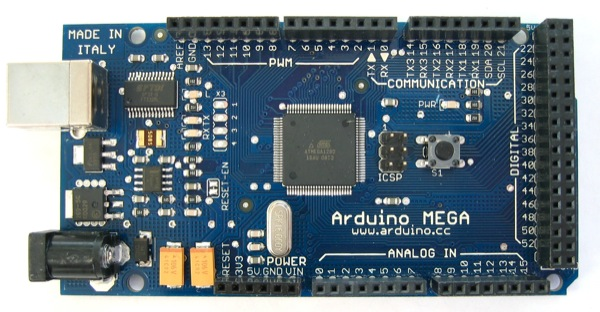
\includegraphics[width=100mm]{img/ArduinoMega.jpg}
\caption[Arduino Mega 2560]{Arduino Mega 2560}\label{ardu}
\end{figure}

\subsection{Temperatursensoren}\thispagestyle{empty}

Vergleich des Stromes durch eine 100 Ohm Präzisionswiderstand (Temperaturstabilität!) mit dem Strom durch einen PT-100. Als Stromquelle diente eine REF200-Stromquelle, welche 2 mal 100 Mikroampere (+- 0.5 Prozent) liefert.

\begin{figure}[htbp]
\centering
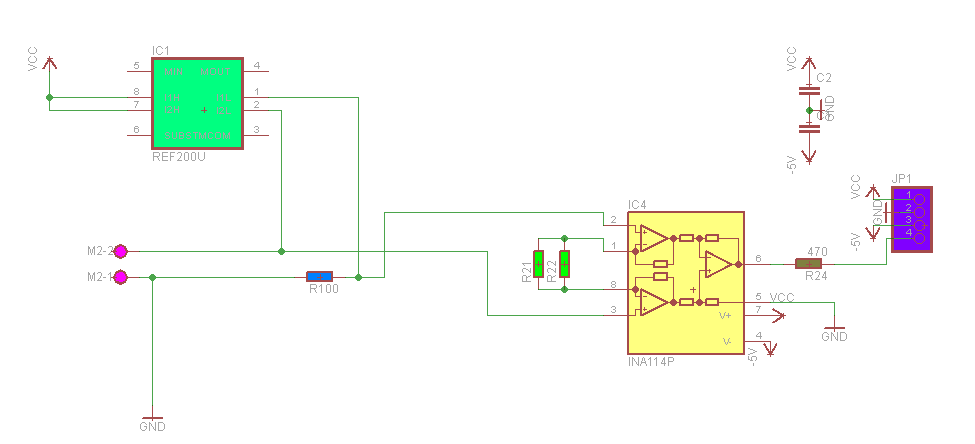
\includegraphics[width=100mm]{img/tmess.png}
\caption{Schaltung der Temperaturmessung}\label{tmess}
\end{figure}

\begin{figure}[htbp]
\centering
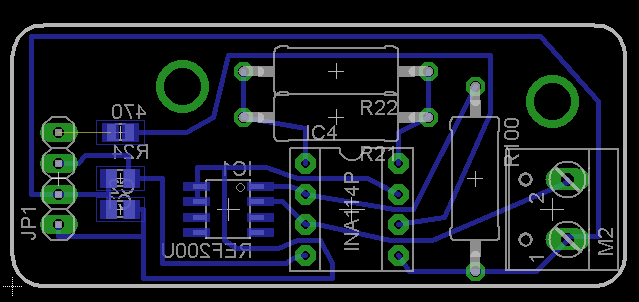
\includegraphics[width=100mm]{img/tmess2.png}
\caption[Arduino Mega 2560]{Layout der Temperarurmessung}\label{tmess2}
\end{figure}


\section{Softwareentwicklung}\thispagestyle{empty}
\subsection{Entwicklungsumgebung}\thispagestyle{empty}
The microcontroller on the board is programmed using the Arduino programming language (based on Wiring) and the Arduino development environment (based on Processing). Arduino projects can be stand-alone or they can communicate with software running on a computer (e.g. Flash, Processing, MaxMSP). 
\begin{figure}[htbp]
\centering
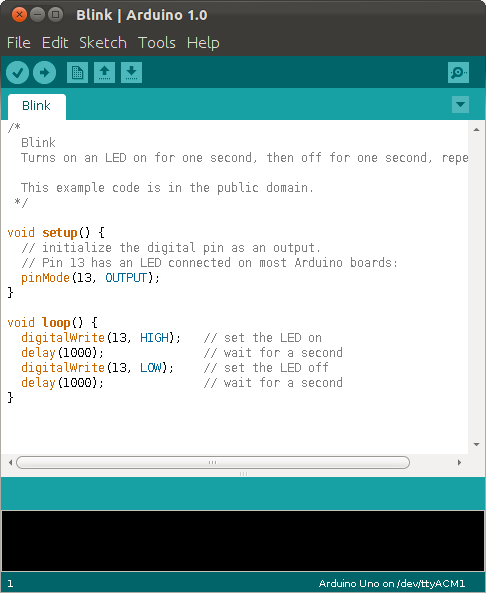
\includegraphics[width=75mm]{img/Arduino.png}
\caption[Arduino Entwicklungsumgebung]{Arduino Entwicklungsumgebung}\label{ardu2}
\end{figure}


\subsection{Auswertung optische sensoren}\thispagestyle{empty}
Differentielle Messung: Zwar liegen die optischen Sensoren auf der Unterseite des Roboters, aber da es im Sonnensimulator eine Einstrahlung von 1000 Watt pro Quadratmeter gibt, mit einem Anteil im spektralen Arbeitsbereich der optischen Sensoren CNY70, ist es notwendig den Einfluss des Streulichtes zu unterdrücken. Dazu wird einmal mit und einmal ohne eingeschalteter Infrarot-LED gemessen, dann der Dunkelwert vom Hellwert abgezogen.


Mathematik Auswertung,
Anhand der Werte der einzelnen optischen Sensoren wird die Lage der Linie relativ zum Mittelpunktes des Arrays bestimmt. 
Rohefassung: Die Methode der kleinsten Quadrate (engl.: method of least squares) ist das mathematische Standardverfahren zur Ausgleichungsrechnung. Dabei wird zu einer Datenpunktwolke eine Kurve gesucht, die möglichst nahe an den Datenpunkten verläuft. Die Daten können physikalische Messwerte, wirtschaftliche Größen oder Ähnliches repräsentieren, während die Kurve aus einer parameterabhängigen problemangepassten Familie von Funktionen stammt. Die Methode der kleinsten Quadrate besteht dann darin, die Kurvenparameter so zu bestimmen, dass die Summe der quadratischen Abweichungen der Kurve von den beobachteten Punkten minimiert wird. Die Abweichungen werden Residuen genannt.
\newline
Folge der Linie: Der Roboter fährt standardmäßig gerade aus. Wird ein Versatz zur Linie erkannt, wird dieser Versatz durch eine Bewegung normal zur Linie minimiert. Eine Verdrehung zur Linie wird durch Verdrehen des Roboters korrigiert. Ein minimaler Versatz, bzw. eine minimale Verdrehung ist dabei zulässig. 
Das vorwärts- und rückwärts-Fahren funktioniert dabei besser als das nach rechts-Fahren. Mecanum-Räder haben eine Vorzugsrichtung.

Behandlung der Ecken: 

Ecken müssen als solche erkannt werden, bevor sie die normale Fahrregelung stören.
Wird eine Ecke erkannt wird der normale Fahrmodus unterbrochen, und in einem speziellen Eckenmodus gewechselt.
Es gibt zwei Arten von Ecken: 
- einmal die klassische Ecke beim Wechsel vom Vor- bzw. Rückwärtsfahren nach rechts.
- Die nach Rechts-Fahren Bahn endet, anstatt in einer Ecke in die Vor- bzw. Rückwärtsbahn zu enden.
Damit ist auch das um die Ecke fahren auch unterschiedlich.
Im Vor- bzw. Rückwärts-Fahren wird die Fahrt ohne Regelung solange fortgesetzt bis die obere bzw. untere Zeile der Sensormatrix schwarz sieht, dann fährt der Roboter ohne Regelung einge hundert Millisekunden nach rechts. Erst dann wird in den nach Rechts-Fahr-Modus gewechselt.
Für den Rechts-fahr Modus endet die Linie abrupt. Der Roboter fährt einige hundert Millisekunden vor bzw. zurück. Dann steht er auf der Führungslinie. Bevor in den eigentlichen Vor- bzw. Rückwärtsfahrmodus gewechselt wird, wird der Roboter zur Linie hin ausgerichtet. Die Unterschiedliche Behandlung der Ecken ist notwendig, weil im Rechtsfahren größere Abweichungen von der Ideallinie auftraten als im Vor- und Zurückfahren.

Haltepunkte: Haltepunkte werden mit dem Haltepunktsensor erkannt, wenn dieser den Schwellwert für weiß überschreitet. Damit ein Haltepunkt nicht mehrfach erkannt werden kann, gibt es eine Verriegelung in der Software, die einen neuen Haltepunkt erst wieder zulässt wenn der Haltepunktsensor in der zwischen Zeit schwarz gesehen hat.



\subsection{Auswertung ADCs}\thispagestyle{empty}
Aufgrund von Rauschen der ADC-Werte, wurden alle Messwerte über 500 Einzelmessungen gemittelt. Der notwendige Messzeit dafür beträgt unter einer halben Sekunde. 

\subsection{Programmablauf}\thispagestyle{empty}
Das Programm startet im Modus Start, der Roboter steht, und wartet 60 Sekunden, eine Pufferzeit damit nach dem Einschalten des Roboters die Lade des Sonnensimulator hineingeschoben und die Klappe geschlossen werden kann.
Nach Ablauf dieser 60 Sekunden wechselt das Programm in den Modus Vorwärts. In diesem Modus fährt der Roboter in Vorwärtsrichtung. Abweichungen von der Idealspur werden erkannt und korrigiert. Wird mit dem Stopsensor eine Stopmarkierung erkannt, wechselt das Programm in den Messmodus. 



\chapter{Kalibration}\thispagestyle{empty}

Dieses Kapitel beschreibt die Kalibrierung der Messsensoren. Es gibt drei Messplatinen, eine für die Messung des Kurzschlussstromes, und zwei identisch aufgebaute Messplatinen zur Messung der Zelltemperatur beziehungsweise der Umgebungstemperatur. Die Strom-Messplatine wandelt den Kurzschlussstrom der Messzelle in eine Spannung um, welche größenmäßig in einem für den ADC des Arduino auswertbaren Bereich (0 bis 5 Volt) ist. Die beiden Messschaltungen zur Temperaturmessung wandeln die Größe der temperaturabhängigen Messwiderstände, jeweils ein Pt-100, in eine Spannung um.
Die ADC-Messwerte wurden über die USB-Schnittstelle des Roboters ausgelesen. Dafür benötigt der Roboter ein einfaches Kalibrierprogramm, welches die gemessenen und gemittelten ADC-Werte über die USB-Schnitstelle sendet. 



\section{Temperatursensoren}\thispagestyle{empty}
Zur Temperaturmessungen werden zwei Pt100 Messfühler verwendet. Die Temperatur der Messzelle wird mit einem an die Messzelle von unten aufgeklebten flächigen Folienmesswiderstand gemessen. 
Ein zweiter Pt100, in kompakter Dünnschichtbauweise ausgeführt, misst die Temperatur der Umgebung. Beide Messschaltungen sind identisch aufgebaut, dennoch können Bauteiltoleranzen zu leicht unterschiedlichen Messspannungen führen.
Für die Kaltbration der Temperaturmesselektronik wurden die Pt-100 Widerstände durch einen hoch genaues, einstellbares und kalibriertes Messnormal ersetzt. Der Widerstand wurde im Bereich von 100 bis 122 Ohm in 1 Ohm Schritten verändert, was einer Temperatur von 0 bis 55 $^{\circ}$C entspricht. Die ADC-Werte wurden über die USB-Schnittstelle des Arduino ausgelesen. Es zeigte sich, dass die beiden Schaltungen leicht unterschiedliche Verstärkungen haben. Daher mussten jede Temperaturmessschaltung separat kalibriert werden.  

\begin{table}[htbp]
\centering
\begin{tabular}{ | c | c | }\hline
{\bf R in Ohm} & {\bf ADC Wert}\\ \hline
\hline
101 & 12\\ \hline
102 & 52,5\\ \hline
103 & 92,5\\ \hline
104 & 133\\ \hline
105 & 172,5\\ \hline
106 & 212\\ \hline
107 & 252,5\\ \hline
108 & 292,5\\ \hline
109 & 332\\ \hline
110 & 373,5\\ \hline
111 & 412\\ \hline
112 & 454\\ \hline
113 & 493\\ \hline
114 & 533\\ \hline
115 & 573\\ \hline
116 & 613\\ \hline
117 & 653\\ \hline
118 & 694\\ \hline
119 & 733,5\\ \hline
120 & 775\\ \hline
121 & 815\\ \hline
122 & 857\\ \hline
\end{tabular}
\caption{Die Messwerte der Kalibrierung Messschaltung A}\label{TabA}
\end{table}

Obwohl der 10-Bit ADC des Arduino einen Maximalwert von 1023 hat, ist bedingt durch den Einsatz des Instrumentenverstärkers INA114, der maximale ADC-Wert bei 857, was einer Spannung von 4,18V entspricht.  


\begin{figure}[htbp]
\centering
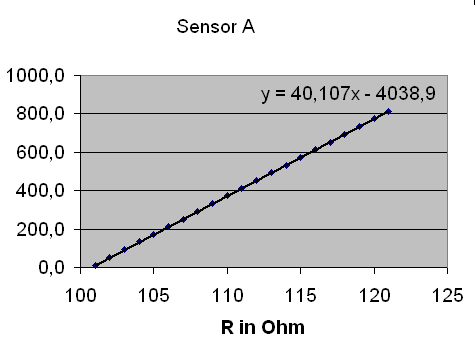
\includegraphics[width=100mm]{img/messa.png}
\caption{Ausgleichsgerade Temperaturmessung A}\label{messa}
\end{figure}

\begin{table}[htbp]
\centering
\begin{tabular}{ | c | c | }\hline
{\bf R in Ohm} & {\bf ADC Wert}\\ \hline
\hline
100 & 0\\ \hline
101 & 20\\ \hline
102 & 59,5\\ \hline
103 & 99\\ \hline
104 & 139\\ \hline
105 & 179\\ \hline
106 & 219\\ \hline
107 & 259\\ \hline
108 & 299\\ \hline
109 & 339\\ \hline
110 & 379\\ \hline
111 & 419,5\\ \hline
112 & 460\\ \hline
113 & 499\\ \hline
114 & 539\\ \hline
115 & 579\\ \hline
116 & 619\\ \hline
117 & 659\\ \hline
118 & 700\\ \hline
119 & 740\\ \hline
120 & 780\\ \hline
121 & 820\\ \hline
122 & 857\\ \hline
\end{tabular}
\caption{Die Messwerte der Kalibrierung Messschaltung B}\label{TabB}
\end{table}

\begin{figure}[htbp]
\centering
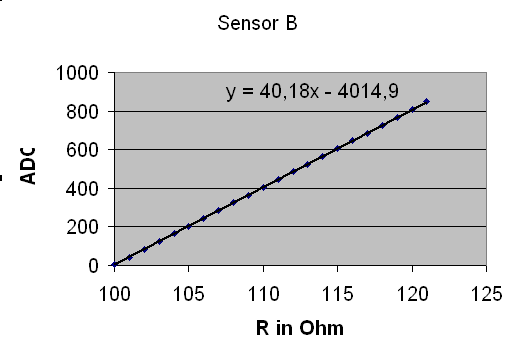
\includegraphics[width=100mm]{img/messb.png}
\caption{Ausgleichsgerade Temperaturmessung B}\label{messb}
\end{figure}

Die gewonnen Formeln für Messschaltung A~\ref{messa} und B~\ref{messa} werden verwendet um aus den ADC-Werten die dazugehörigen Widerstandswerte zu berechnen. 

  \begin{equation}
     R_A(ADC) = \frac{ADC_A + 4039,9}{40,107}
  \end{equation}
  
    \begin{equation}
     R_B(ADC) = \frac{ADC_B + 4039,9}{40,107}
  \end{equation}


\section{Messzelle}\thispagestyle{empty}


Der Kurzschlussstrom der Messzelle wurde im Flasher~\ref{zelleflasher} über einen weiten Temperaturbereich gemessen~\ref{tempkoef}. Es wurde mit der Berger Messlast gemessen. Bei der Messung wurden die Leitungswiderstände der Messkabel minimiert, indem Kabel mit hohem Querschnitt ($6mm^2$) verwendet wurden, und die Kabel möglichst kurz gehalten wurden (<1,5m).
 
\begin{figure}[htbp]
\centering
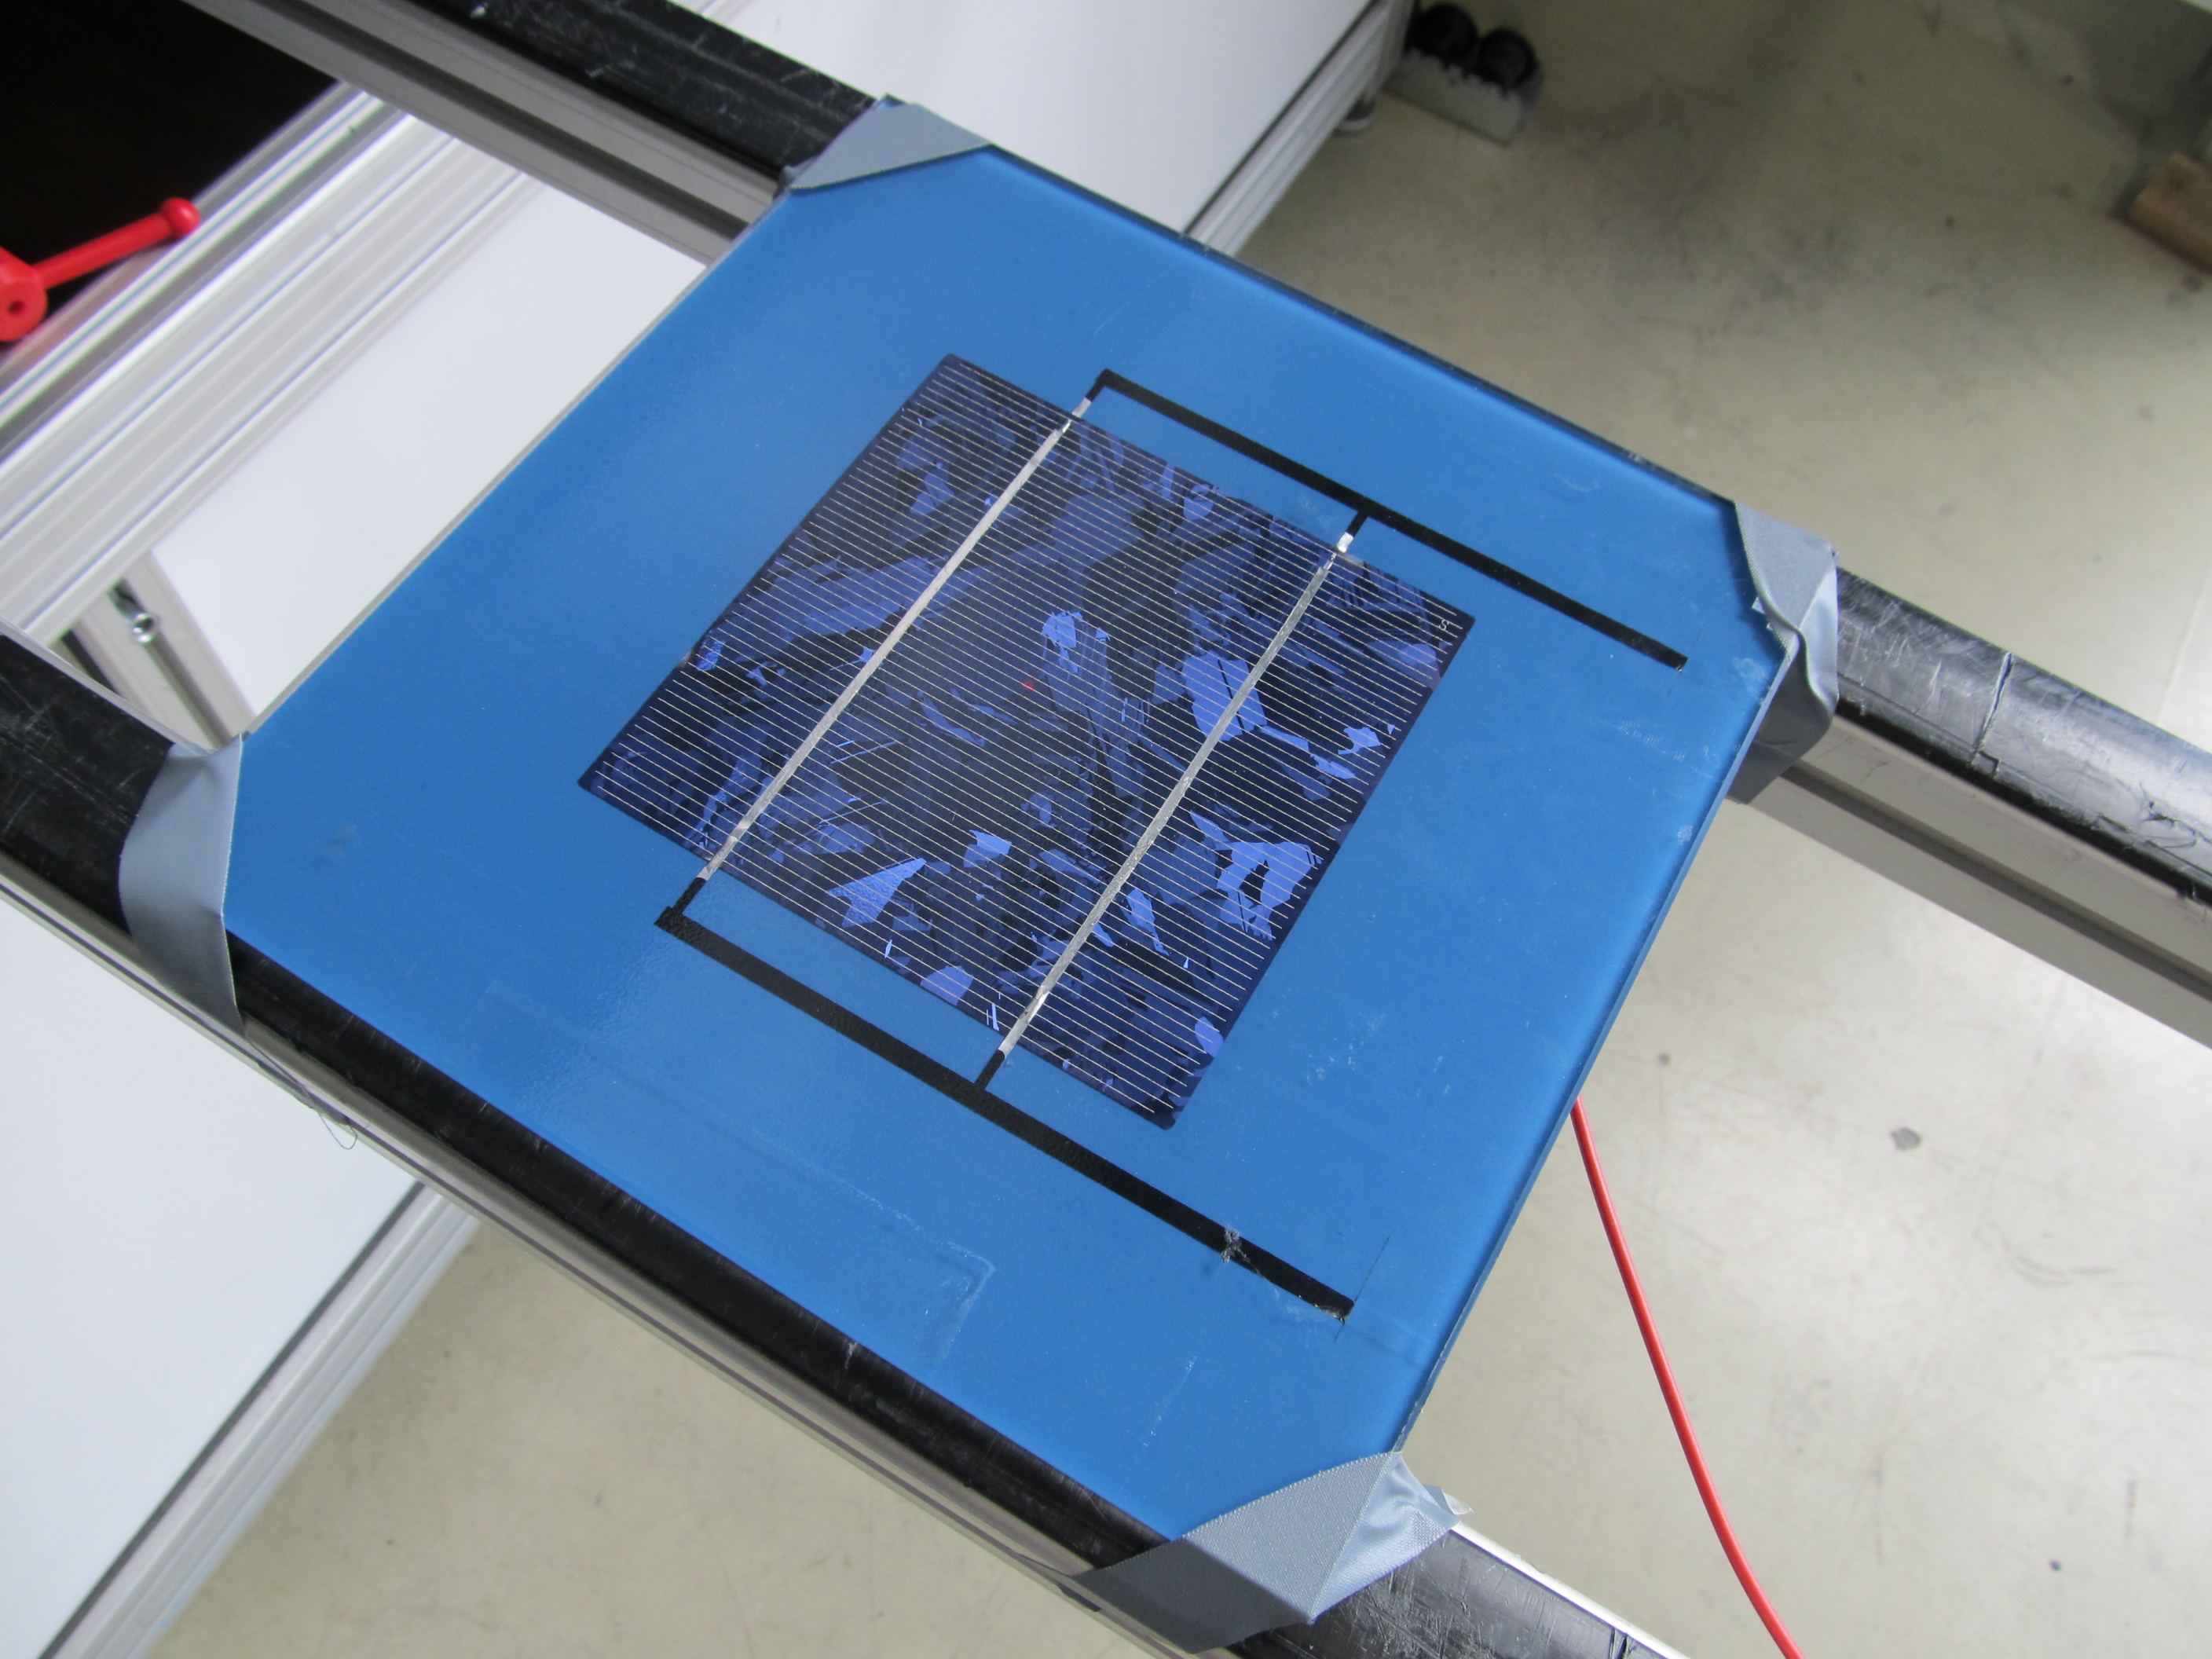
\includegraphics[width=75mm]{img/zelle.jpg}
\caption{Die Messzelle auf dem Einschub des gepulsten Sonnensimualtors}\label{zelleflasher}
\end{figure}

\begin{figure}[htbp]
\centering
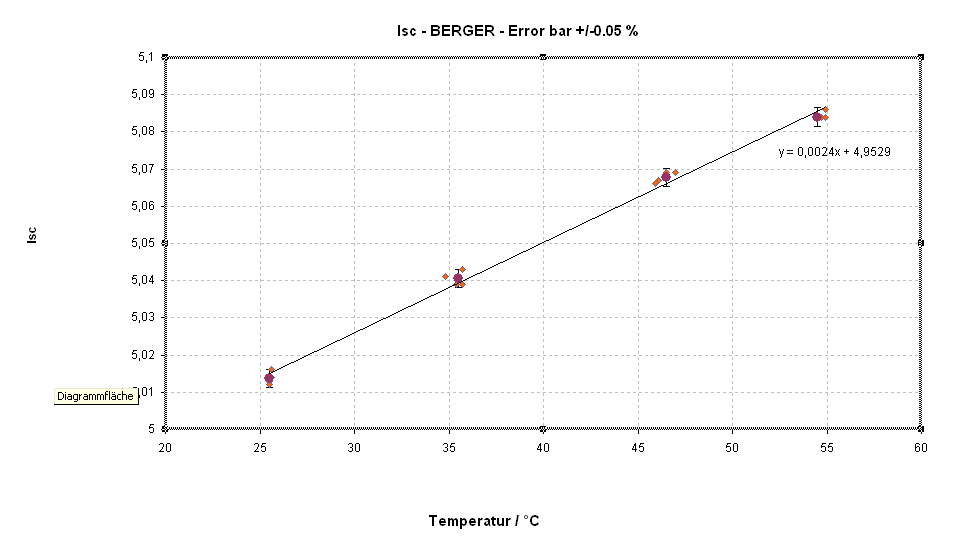
\includegraphics[width=150mm]{img/tempkoef.png}
\caption{Abhängigkeit des Kurzschlussstromes von der Temperatur}\label{tempkoef}
\end{figure}

  \begin{equation}
     I(T) = 4,9529+0.0024 \ast T
  \end{equation}
  
    \begin{equation}
     I(T) = 4,9529 \ast ( 1 + 0,00048 \ast T)
  \end{equation}

\section{Strommessung}\thispagestyle{empty}

Der Messroboter wurde für die Kalibrierung der Strommessung in eine Klimazelle platziert.  Die Temperatur der Klimazelle wurde im Bereich von 8 bis 35 $^{\circ}$C variiert. Durch den Messwiderstand der Strommessung wurde ein Strom im Bereich von 3 bis 8 A geschickt.  

\begin{table}[htbp]
\centering
\begin{tabular}{|l|l|l|}
\hline
T/$^{\circ}$C & I/mA & ADC Wert \\ 
\hline
\hline

\multirow{3}{*}{24,4} & 3997 & 472 \\
 & 6001 & 712 \\
 & 8002 & 854 \\ \hline
\multirow{3}{*}{35,3} & 3999 & 473 \\
 & 6001 & 712 \\
 & 7999 & 859 \\ \hline
\multirow{3}{*}{35,3} & 3999 & 472 \\
 & 6001 & 710 \\
 & 8001 & 852 \\ \hline
\multirow{5}{*}{16,4} & 2004 & 234 \\
 & 3005 & 353 \\
 & 4003 & 473 \\
 & 5003 & 591 \\
 & 6005 & 711 \\ \hline
\multirow{5}{*}{8} & 1993 & 233 \\
 & 2995 & 352 \\
 & 4001 & 472 \\
 & 5000 & 590 \\
 & 6005 & 710 \\ \hline
\end{tabular}
\caption{Kalibrierung Strommessung}\label{TabS}
\end{table}

\begin{figure}[htbp]
\centering
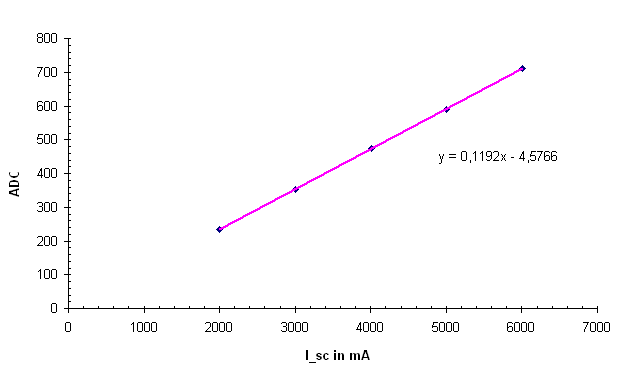
\includegraphics[width=150mm]{img/16grad.png}
\caption{Lineraer Zusammenhang zwischen Strom und dem ADC-Wert}\label{ical}
\end{figure}

\begin{equation}
     I(ADC) = \frac{ADC + 4,5766} {119,2} 
\end{equation}
  


\section{Thermische Stabilität der Temperaturmessung}\thispagestyle{empty}
Zur Bestimmung der Temperaturstabilität wurde der gesamte Roboter in ein Klimakammer gestellt. Der Pt100 wurde durch einen temperaturstabilen 110$\Omega$ simuliert.
Es gab zwei Durchgänge dieses Versuches.
Bei der ersten Messung zeigte sich, dass eine der beiden Messplatinen nicht temperaturstabil war. Durch das Tauschen der Ref200 Stromquelle dieser Platine konnte das Problem gelöst werden.

\begin{table}[htbp]
\centering
\begin{tabular}{ | c | c | c |}\hline
{\bf T in $^{\circ}$C} & {\bf ADC Platine A} & {\bf ADC Platine B}\\ \hline
\hline
11,7 & 368 & 407\\ \hline
13,0 & 368 & 406\\ \hline
13,7 & 368 & 406\\ \hline
14,5 & 368 & 405\\ \hline
15,5 & 368 & 405\\ \hline
16,6 & 368 & 405\\ \hline
17,5 & 368 & 404\\ \hline
23,5 & 368 & 403\\ \hline
27,5 & 368 & 402\\ \hline
\end{tabular}
\caption{Temeraturabhängigkeit der Temperaturmessung}\label{TabT1}
\end{table}

\begin{table}[htbp]
\centering
\begin{tabular}{ | c | c | c |}\hline
{\bf T in $^{\circ}$C} & {\bf ADC Platine A} & {\bf ADC Platine B}\\ \hline
\hline
30,7 & 368 & 380\\ \hline
20,1 & 368 & 379\\ \hline
9,2 & 368 & 378\\ \hline
\end{tabular}
\caption{Temeraturabhängigkeit der Temperaturmessung}\label{TabT1}
\end{table}

Durch den Austausch der Referenzstromquelle der Platine B hat sich auch der ADC-Wert gegenüber der ersten Messung geändert. Die Kalibrierwerte der Platine B \ref{TabB} sind nach diesem Austausch aufgenommen worden.
Da die Platine A temperaturstabiler als die Platine B ist, wurde Platine A zur Messung der Zelltemperatur ausgewählt, die Platine B wurde für die Messung der Umgebungstemperatur verwendet. 







\chapter{Messung}\thispagestyle{empty}
\section{Messaufbau}\thispagestyle{empty}
  \subsection{Platten}\thispagestyle{empty}
Im Sonnensimulator 2 Platten. Auf den 3 Platten ist die Messbahn aufgemalt.
Die Platten müssen eng aneinander anliegen. Damit keine zu groß Stufe wegen unschiedlicher Duschbiegung der Platten entsteht ist auf der Rückseite der Holzplatten Aluminiumbleche befestig, auf einer Seite angeschraubt, die danebenliegende Platte liegt darauf.
Da die Breite aller 3 Platten geringer ist als die Breite der Lade des Sonnensimulators, werden, damit die Messungen zu verschiedenen Zeitpunkten verglichen werden können, die Platten so weit wie möglich nach rechts geschoben. Am Rand liegen die Platten auf Aluschienen auf.
\begin{figure}[htbp]
\centering
\includegraphics[width=125mm]{img/messbahn1.png}
\caption[Messbahn auf den Platten]{Messbahn auf den Platten}\label{bahn}
\end{figure}
Die Übergänge der Messbahn von einer Platte zur nächsten sind mit weißem Isolierband  der Breite 14mm zu überbrücken. Beschädigung der Messbahn, welche durch unsanftes Handling der Platten entstehen können, sind ebenfalls mit weißem Isolierband zu Überkleben.





\subsection{Ablauf}\thispagestyle{empty}

Roboter wird auf das linke vordere Ende der Messbahn gestellt. Der Roboter muss dabei auf der Messbahn stehen. Kleinere Abweichungen der Idealposition werden beim losfahren korrigiert. 
Vor der eigentlichen Messfahrt ist eine Testfahrt mit geöffneter Lade des Sonnensimulators zu empfehlen. Besonders die Übergänge von einer Platte zur nächsten können Probleme schaffen.
Nach der bestandenen Testfahrt wird der Sonnensimulator eingeschaltet. Bis zur Messung sind 20 bis 30 Minuten zu warten, bis die Temperaturen im Simulator stabil sind. Der Roboter kann während dieser Zeit im Sonnensimulator stehen. Die Messzelle sollte allerdings abgeschattet werden, damit diese sich nicht aufheizt. 
Zum Starten wird der Schalter von 0 auf 1 umgelegt. Damit wird der Mikrocontroller mit Spannung versorgt. Das Programm startet. Nach einer Pause von 60 Sekunden, die zum Schließen des Sonnensimulators notwendig ist, fährt der Roboter los. Eine Messfahrt dauert etwa 13 Minuten. Nach Ablauf dieser Zeit wird der Roboter entnommen und die Daten der SD-Karte entnommen, oder der Roboter wird auf die Startposition gestellt um weitere Messfahrten durchzuführen.


\section{Auswertung}\thispagestyle{empty}


wie von sd  zu Bild,
gemessene Verteilungen,

Rohfassung: ADC Werte werden auf SD Karte gespeichert:
Zeit in ms, Isc, Temperatur des Moduls, Umgebungstemperatur, Messpunkt, Reihe, Spalte
Es sind 308 Messpunkte, 14 mal 22, es kann vorkommen, am Übergang von einer Platte zur anderen, dass ein Messpunkt ausgelassen wird. Das ist erkennbar wenn nicht 308 Messwerte im datalog-File sind. Um den Fehler leicht zu finden wurde Spalte und Reihe mit aufgezeichnet. Sind in einer Spalte nur 13 Messwerte, fehlt in dieser Spalte ein Wert. Anhand der mit aufgezeichneten Zeit kann der fehlende Messpunktes lokalisiert werden. Das geschiet nicht automatisch Der Messwert wird anhand der neben liegenden Werte geschätzt. Alternativ werden nur Messfahrten mit allen Punkten ausgewertet.

Auf der SD Karte sind alle Messwerte in einer Wurscht gespeichert. Für die visuelle Auswertung wird diese Datenwurst in ein zweidimensionales Array umgewandelt. 
Formel, Formel
Der ADC Wert des Kurschlussstromes wird in Ampere umgerechnet. Verwendet wird die in der Kallibrierung gewonnene Formel.

\begin{figure}[htbp]
\centering
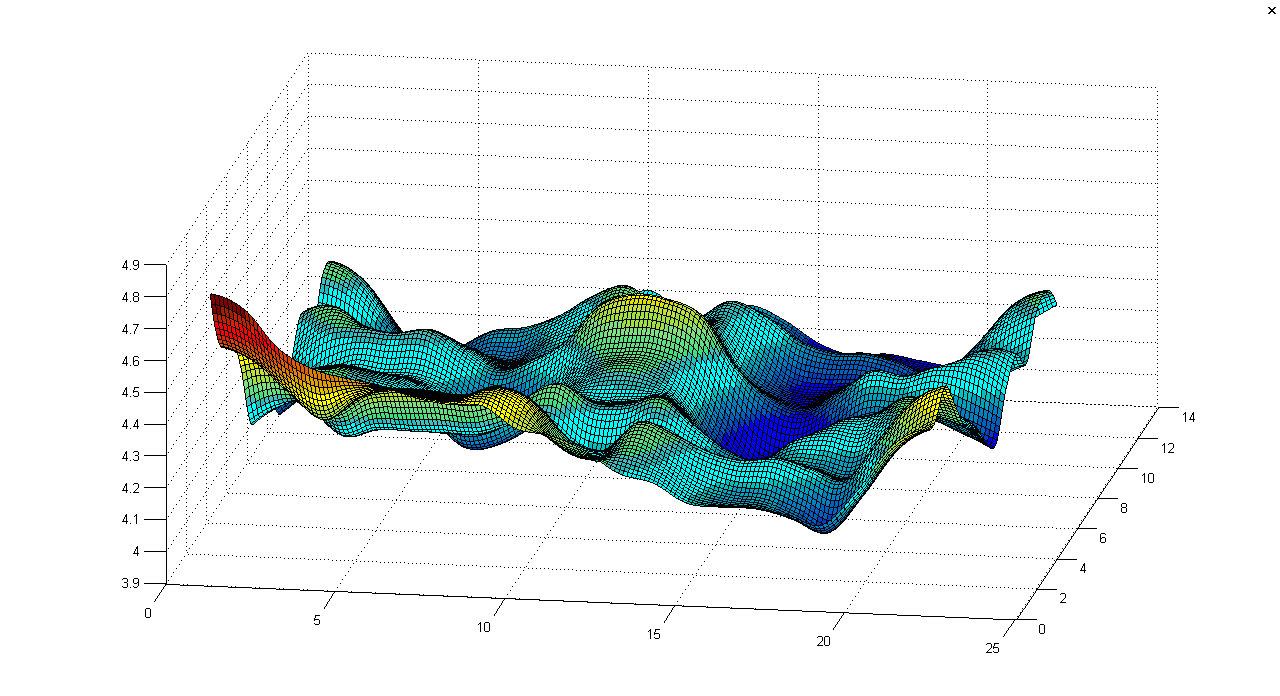
\includegraphics[width=150mm]{img/hugel.png}
\caption[Kurzschlusstrom in Ampere]{Kurzschlusstrom in Ampere}\label{hugel}
\end{figure}



\begin{figure}[htbp]
\centering
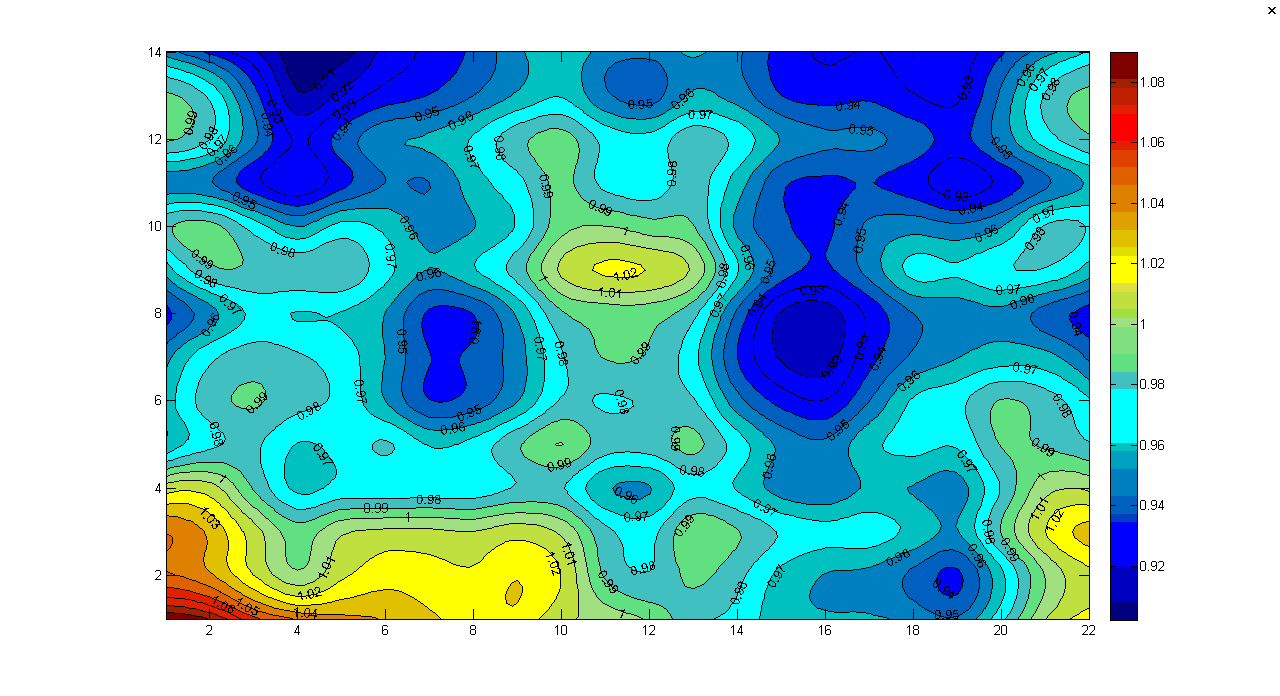
\includegraphics[width=150mm]{img/karte1.png}
\caption[Relative Verteilung der Einstrahlung]{Relative Verteilung der Einstrahlung}\label{karte1}
\end{figure}

\begin{figure}[htbp]
\centering
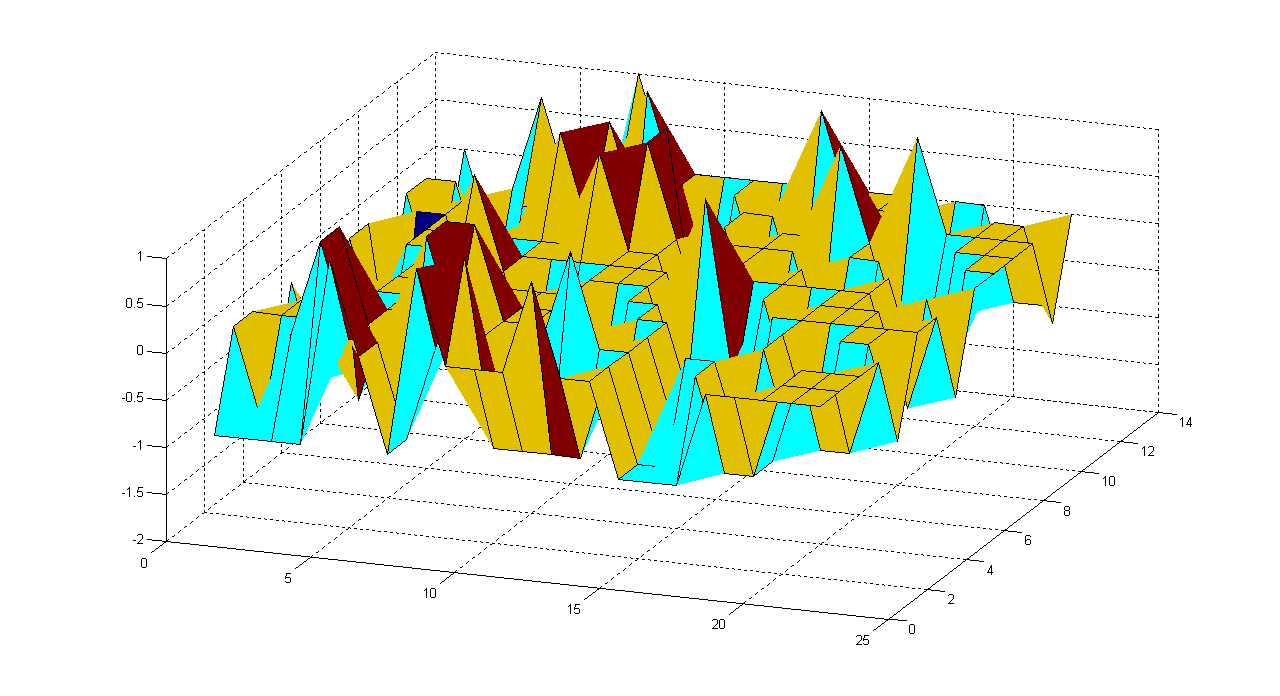
\includegraphics[width=150mm]{img/vergleich23.png}
\caption[Vergleich zweier Messungen]{Vergleich zweier Messungen}\label{vergleich}
\end{figure}

\begin{figure}[htbp]
\centering
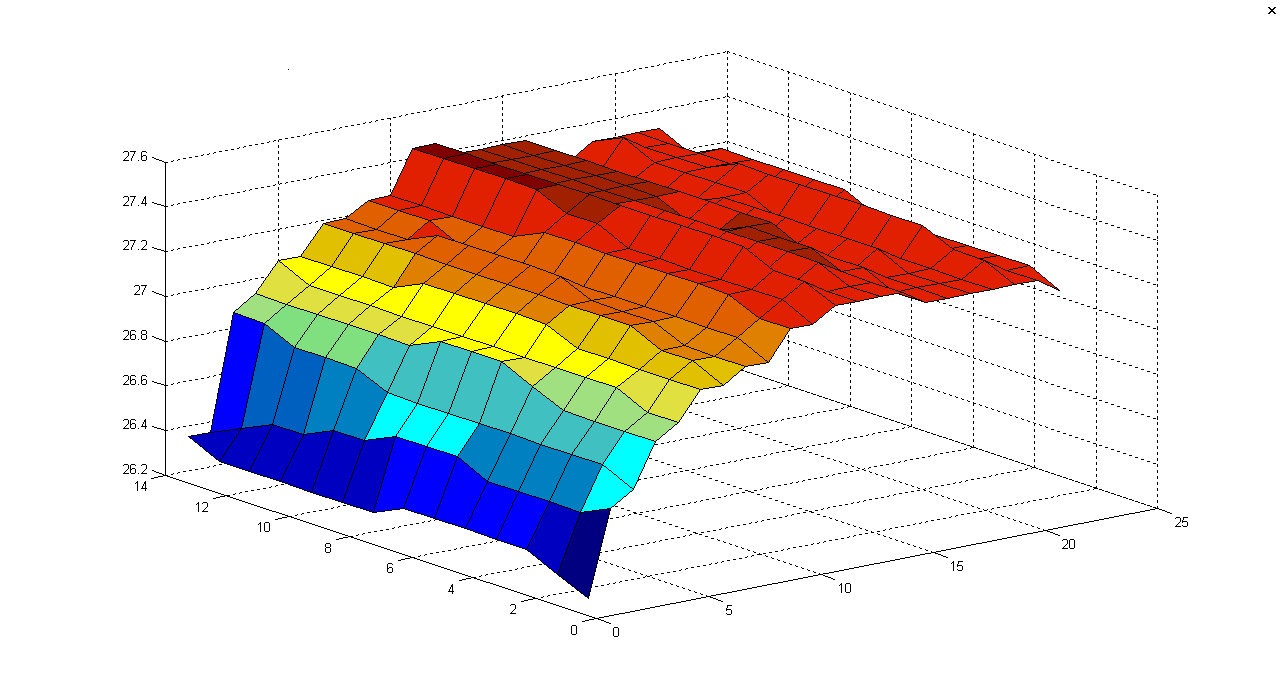
\includegraphics[width=150mm]{img/tempm1.png}
\caption[Temperatur der Zelle]{Temperatur der Zelle}\label{tm1}
\end{figure}

\begin{figure}[htbp]
\centering
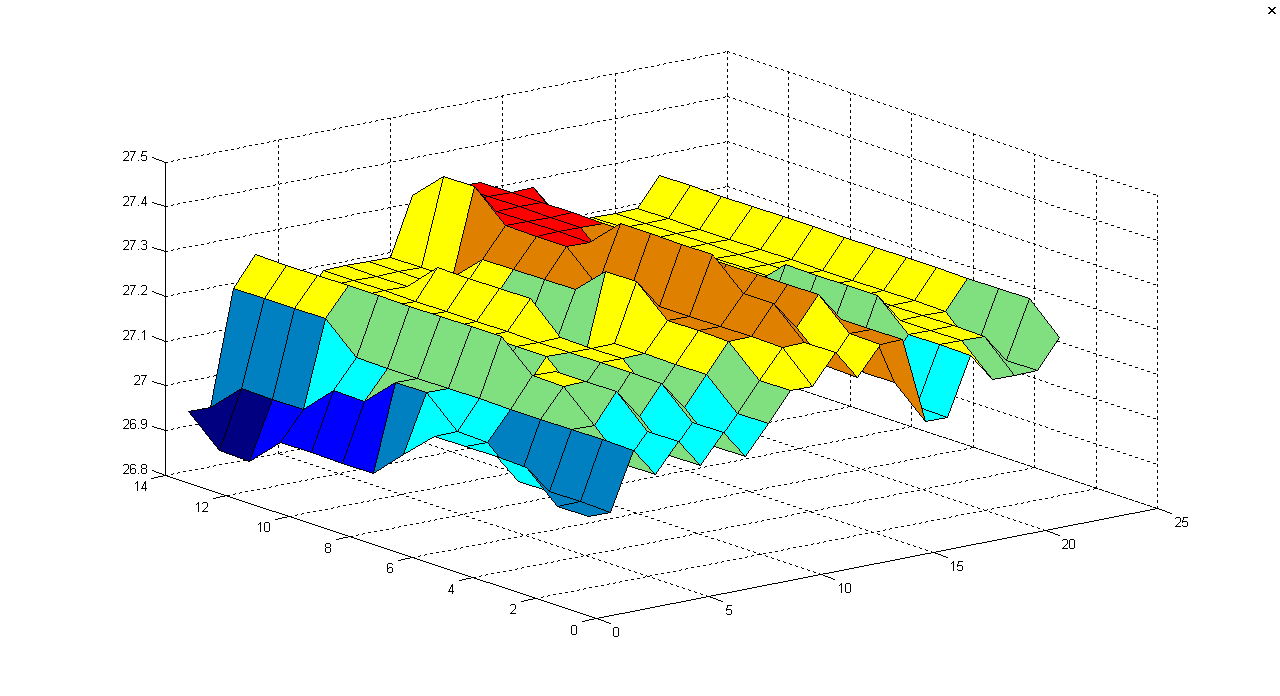
\includegraphics[width=150mm]{img/tempm2.png}
\caption[konstante Temperatur der Zelle]{konstante Temperatur der Zelle}\label{tm2}
\end{figure}


\section{Vermessung der Ausleuchtung einzelner Lampen}

Die geringe Messzeit des Roboters, verglichen mit der mechanischen Methode, macht es möglich die Bestrahlungsstärkeverteilung der einzelnen Lampen in realistischer Zeit zu bestimmen.
Veränderbar sind der Abstand zwischen Lampenfeld und Prüfebene. Die Leistungen der Lampen lassen sich einzeln steuern. 

\begin{figure}
    \subfigure[3D Ansicht]{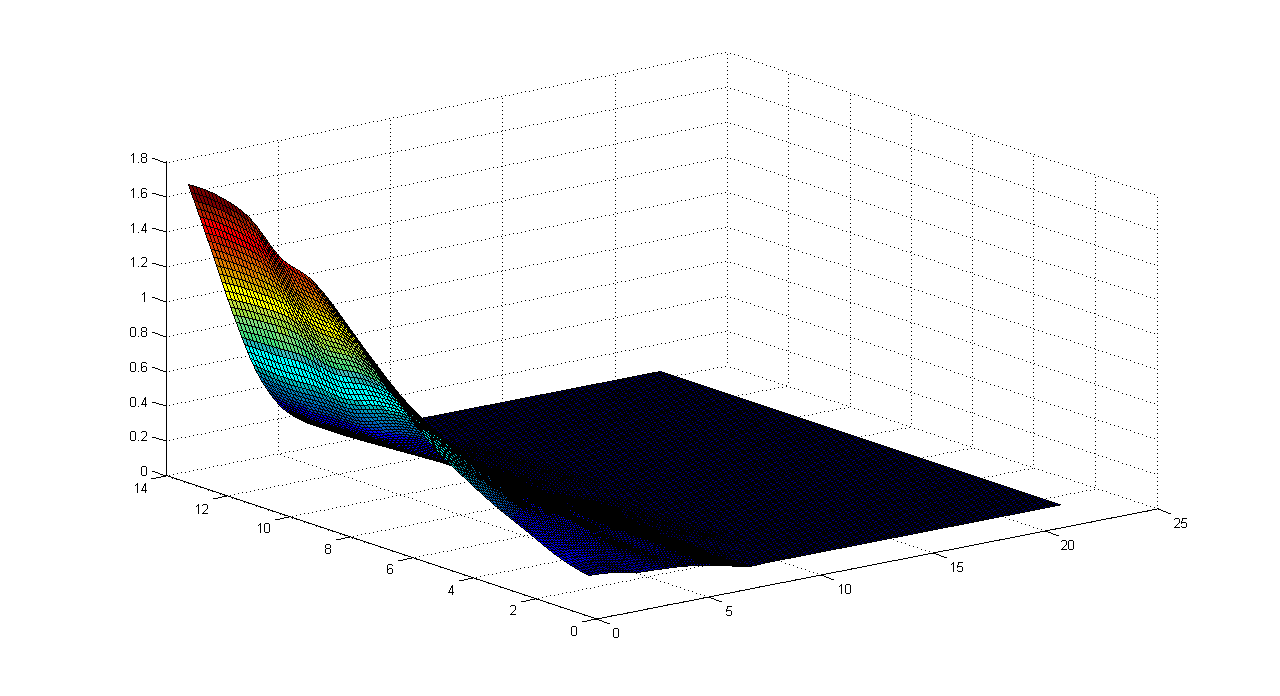
\includegraphics[width=0.49\textwidth]{img/E1.png}}
    \subfigure[Landkarte]{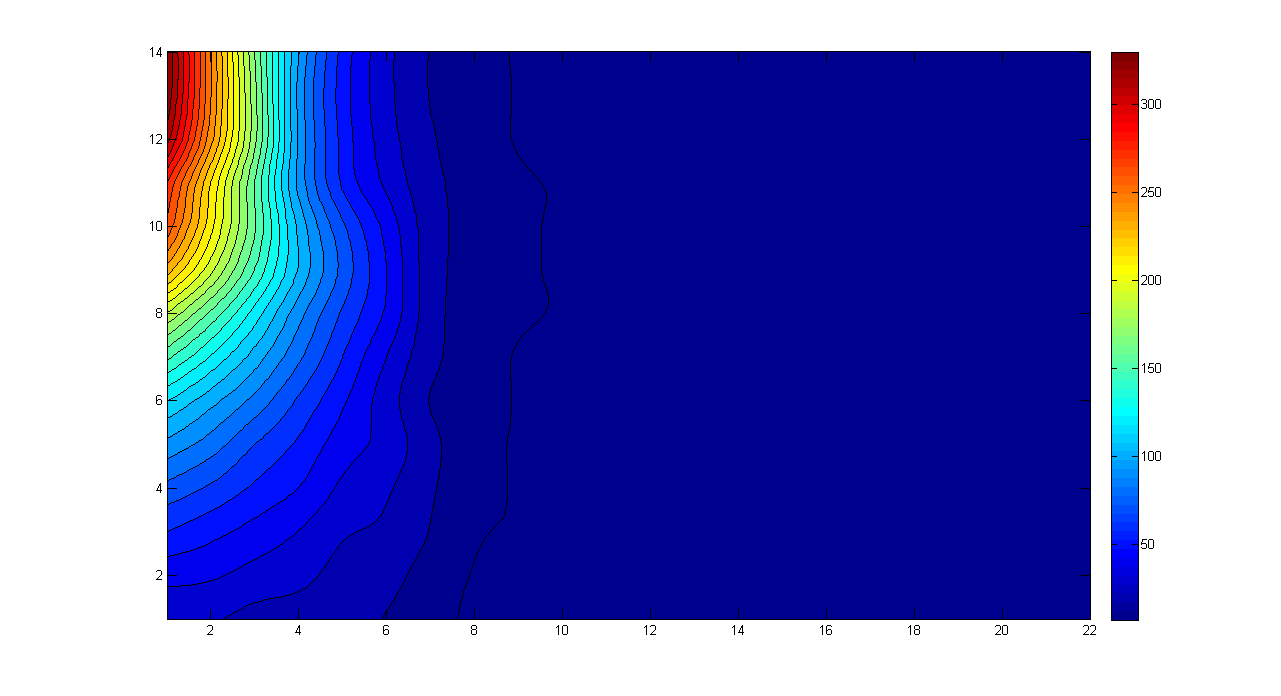
\includegraphics[width=0.49\textwidth]{img/E1a.png}}
\caption{Lampe E1}
\end{figure} 

\begin{figure}
    \subfigure[3D Ansicht]{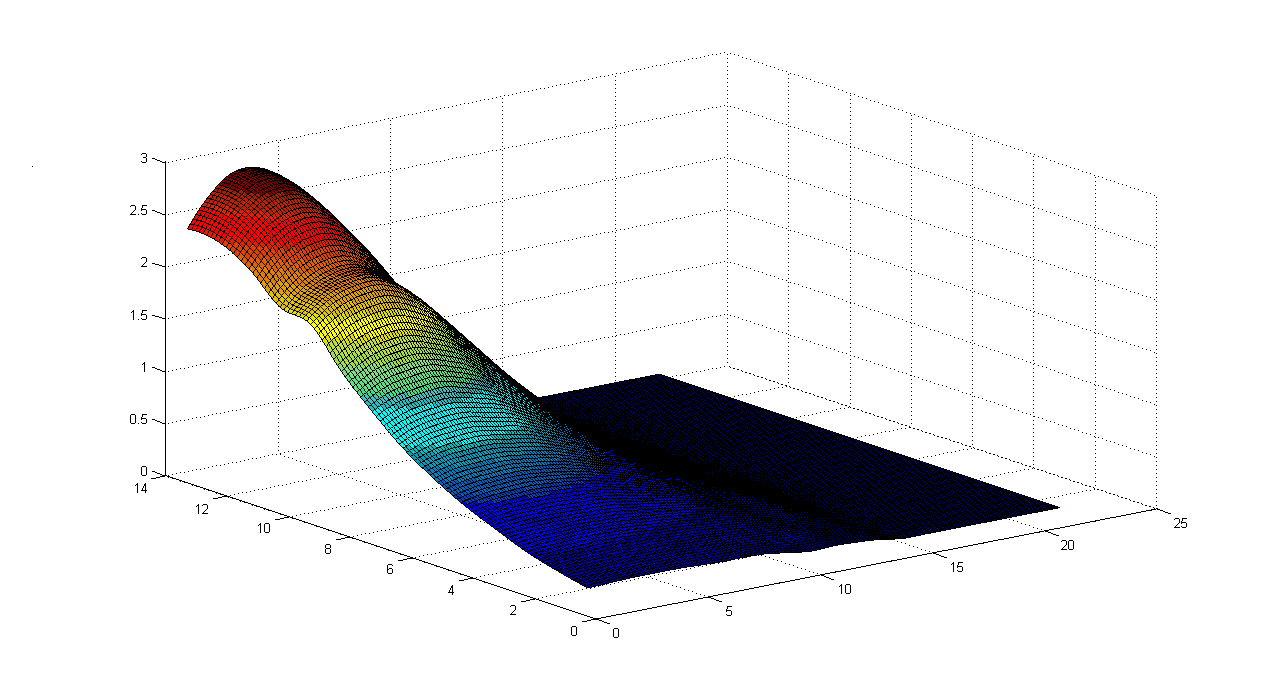
\includegraphics[width=0.49\textwidth]{img/E2.png}}
    \subfigure[Landkarte]{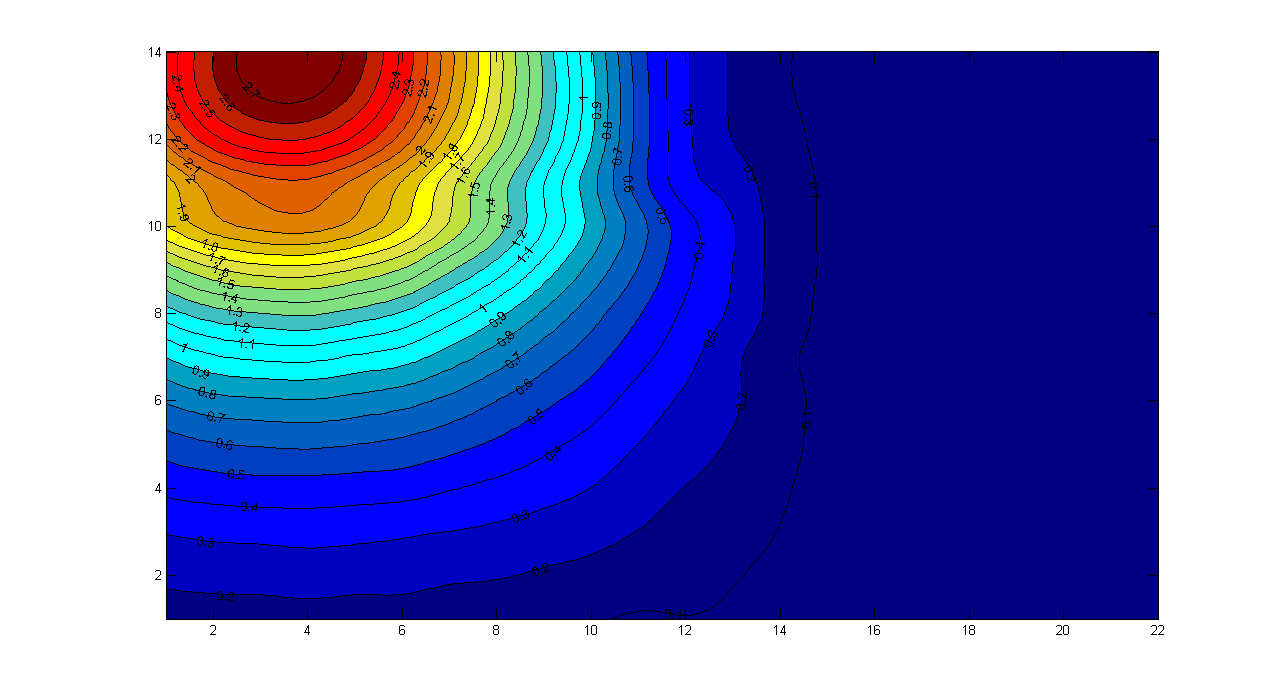
\includegraphics[width=0.49\textwidth]{img/E2a.png}}
\caption{Lampe E2}
\end{figure} 

\begin{figure}
    \subfigure[3D Ansicht]{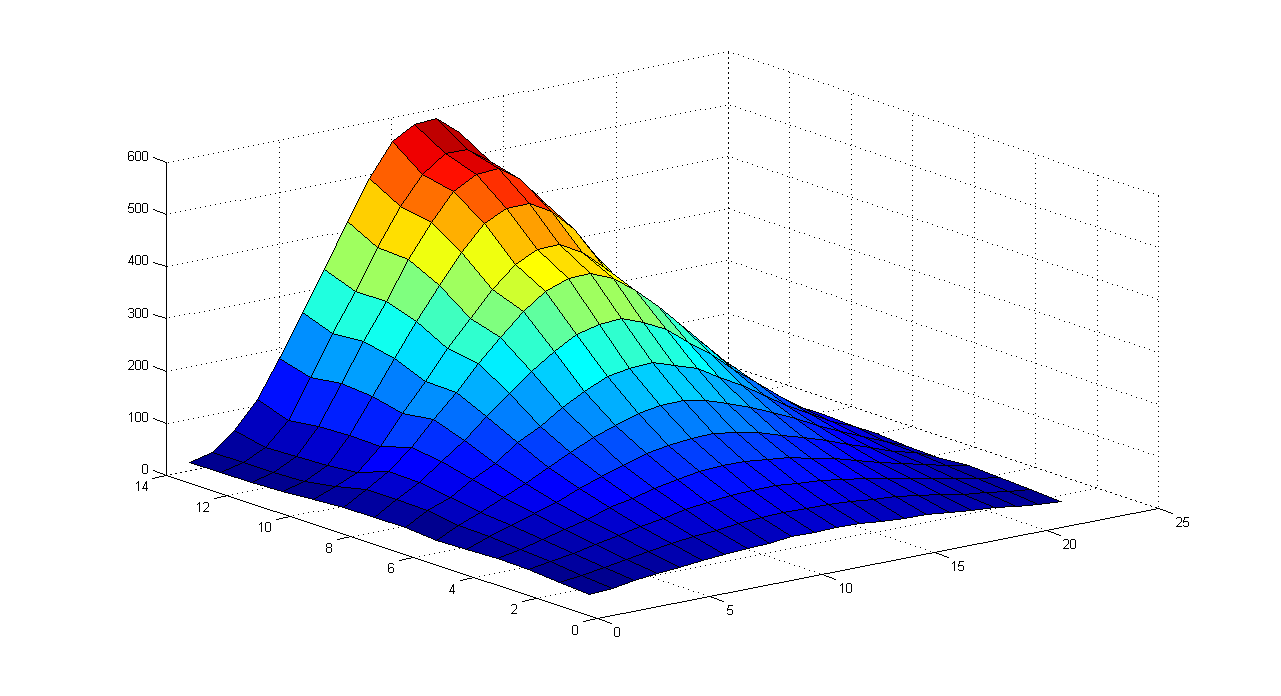
\includegraphics[width=0.49\textwidth]{img/E3.png}}
    \subfigure[Landkarte]{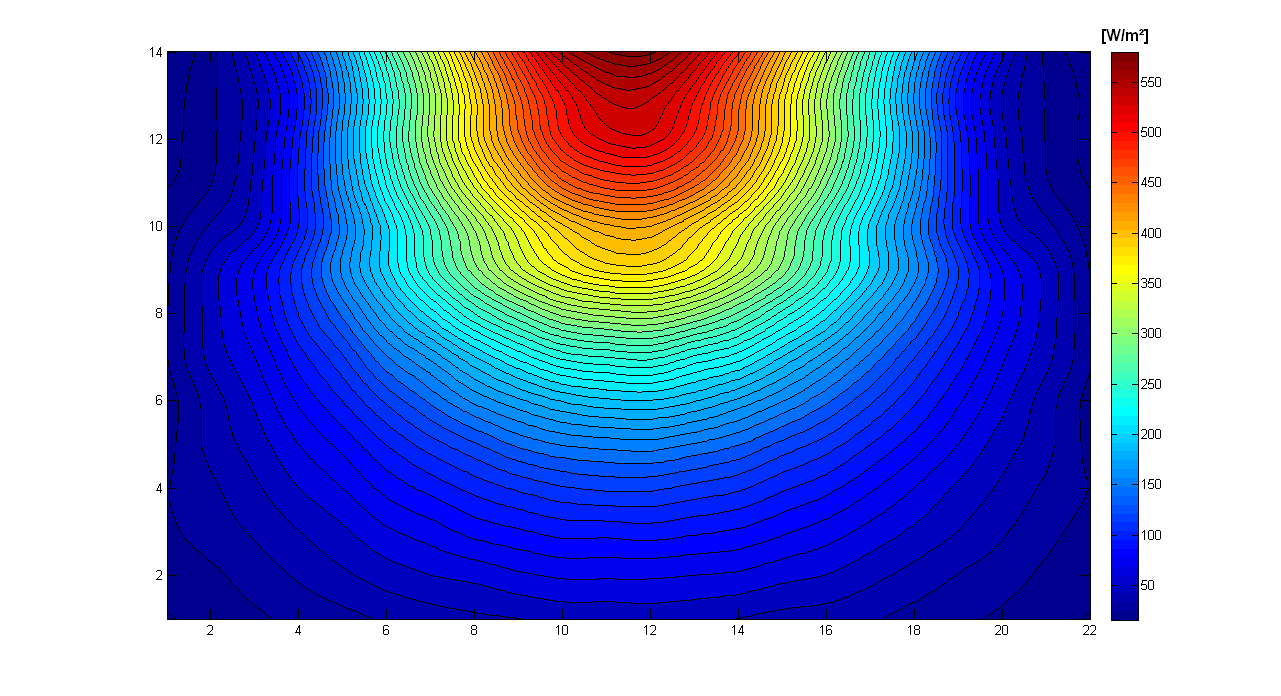
\includegraphics[width=0.49\textwidth]{img/E3a.png}}
\caption{Lampe E3}
\end{figure}

\begin{figure}
    \subfigure[3D Ansicht]{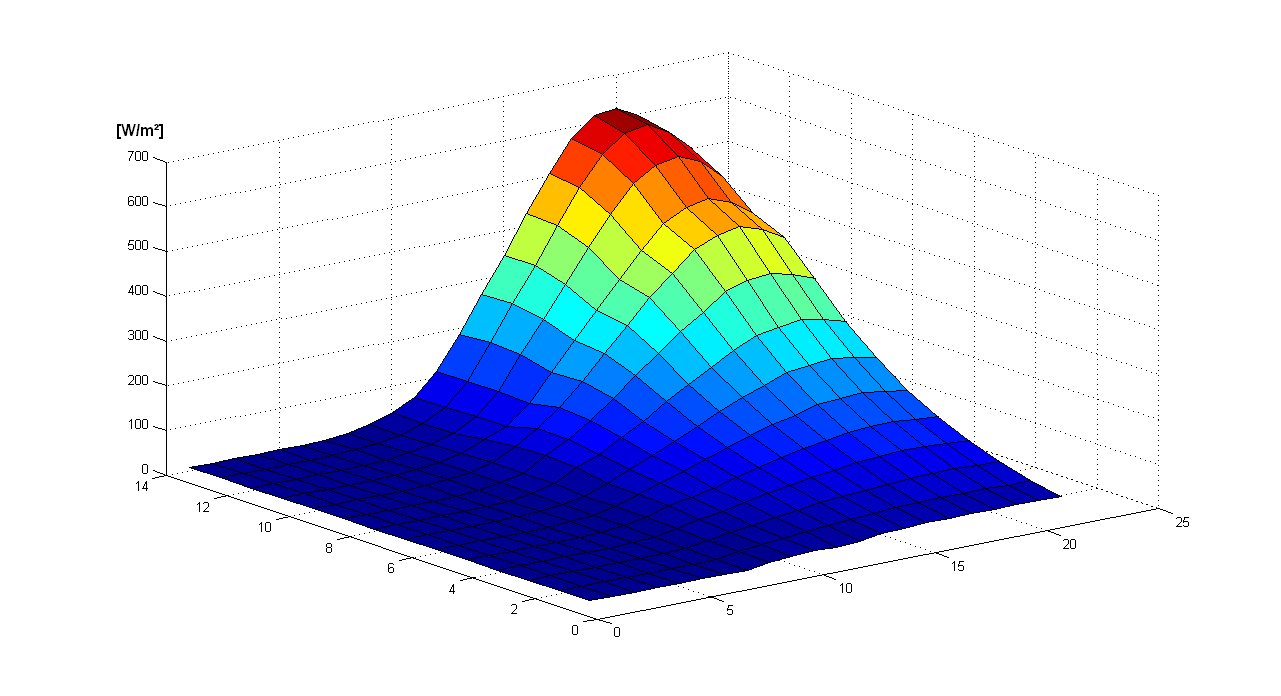
\includegraphics[width=0.49\textwidth]{img/E4.png}}
    \subfigure[Landkarte]{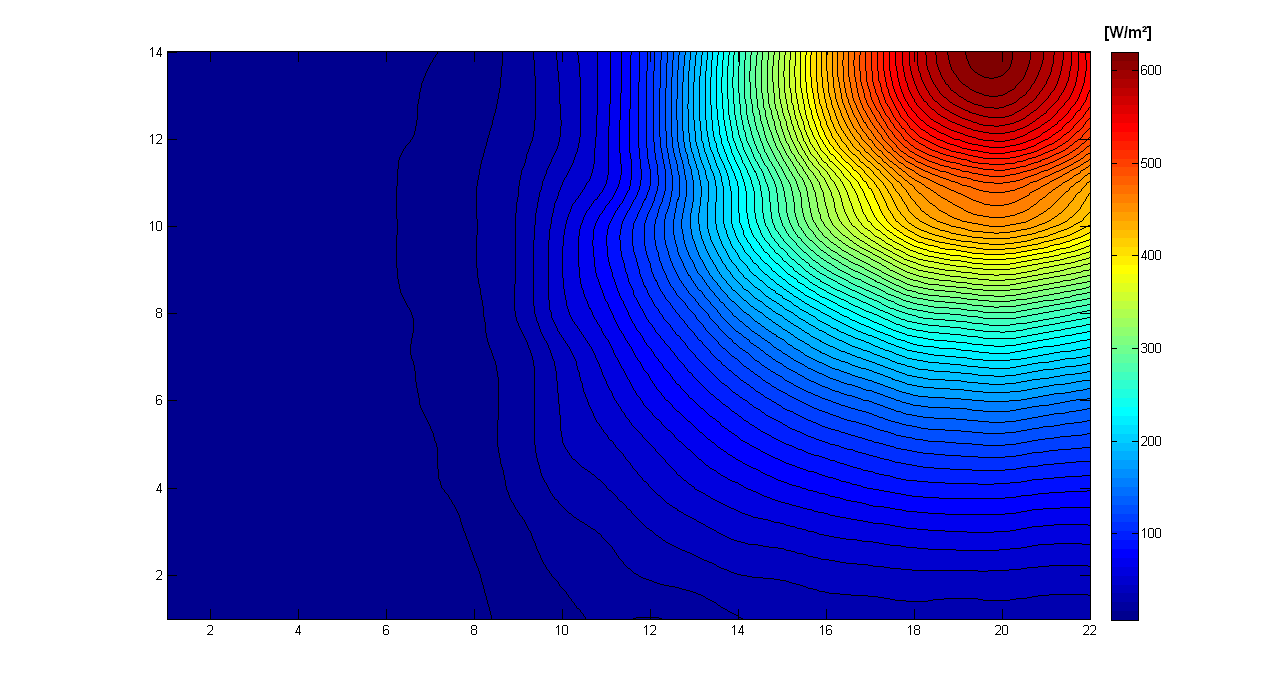
\includegraphics[width=0.49\textwidth]{img/E4a.png}}
\caption{Lampe E4}
\end{figure} 

\begin{figure}
    \subfigure[3D Ansicht]{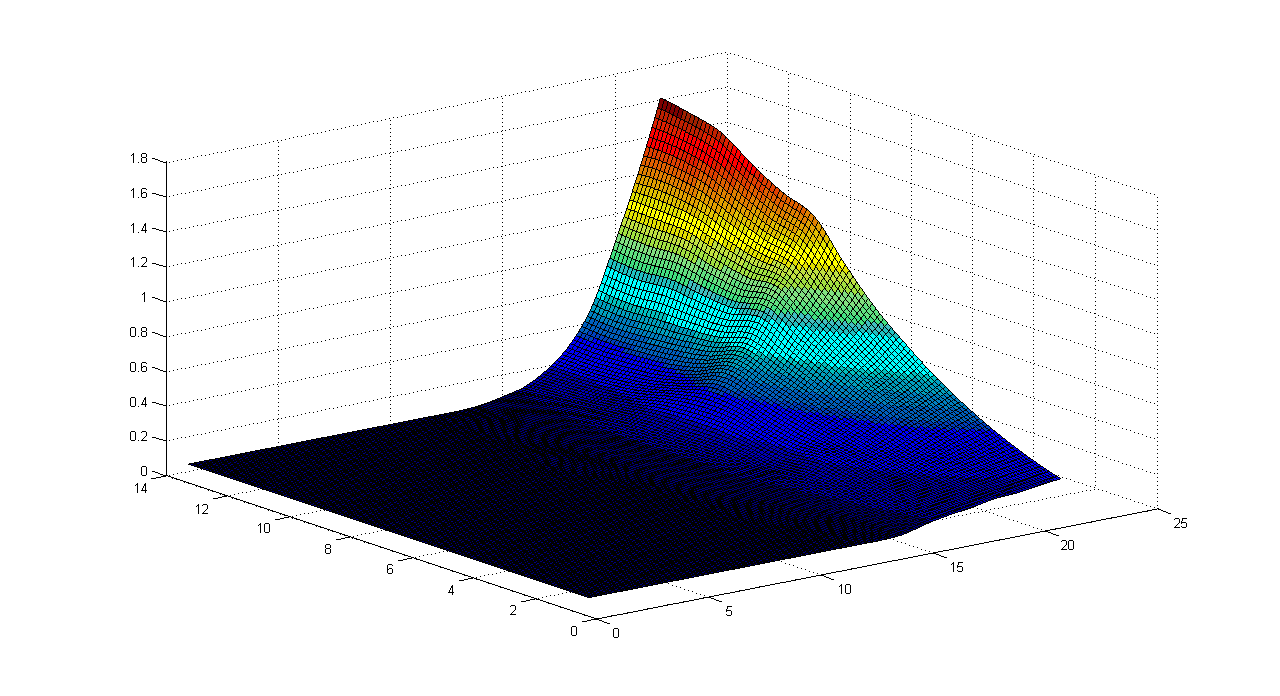
\includegraphics[width=0.49\textwidth]{img/E5.png}}
    \subfigure[Landkarte]{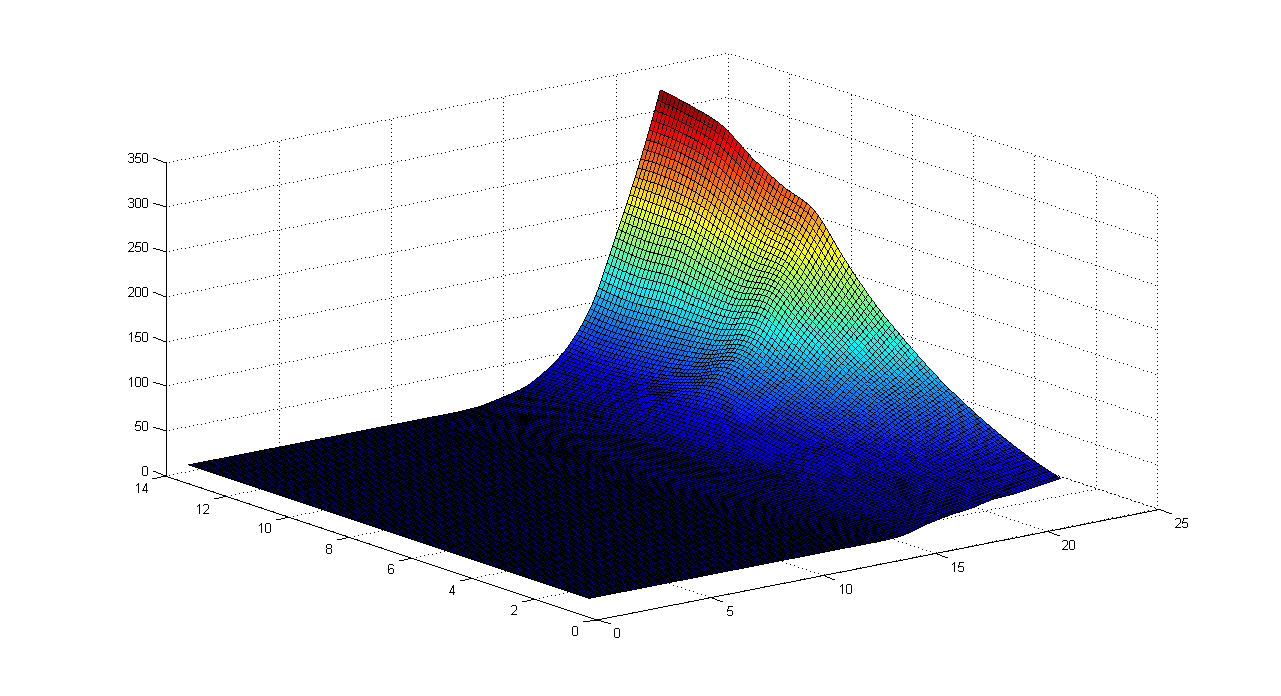
\includegraphics[width=0.49\textwidth]{img/E5a.png}}
\caption{Lampe E5}
\end{figure} 

\begin{figure}
    \subfigure[3D Ansicht]{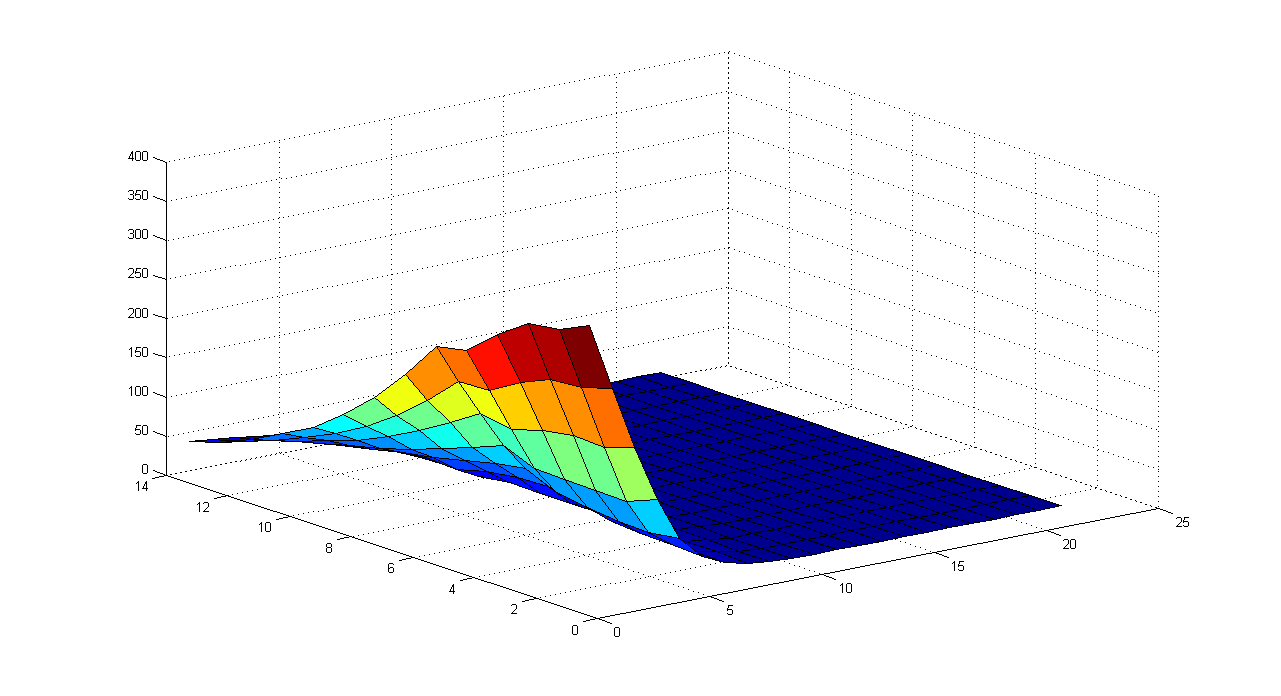
\includegraphics[width=0.49\textwidth]{img/E6.png}}
    \subfigure[Landkarte]{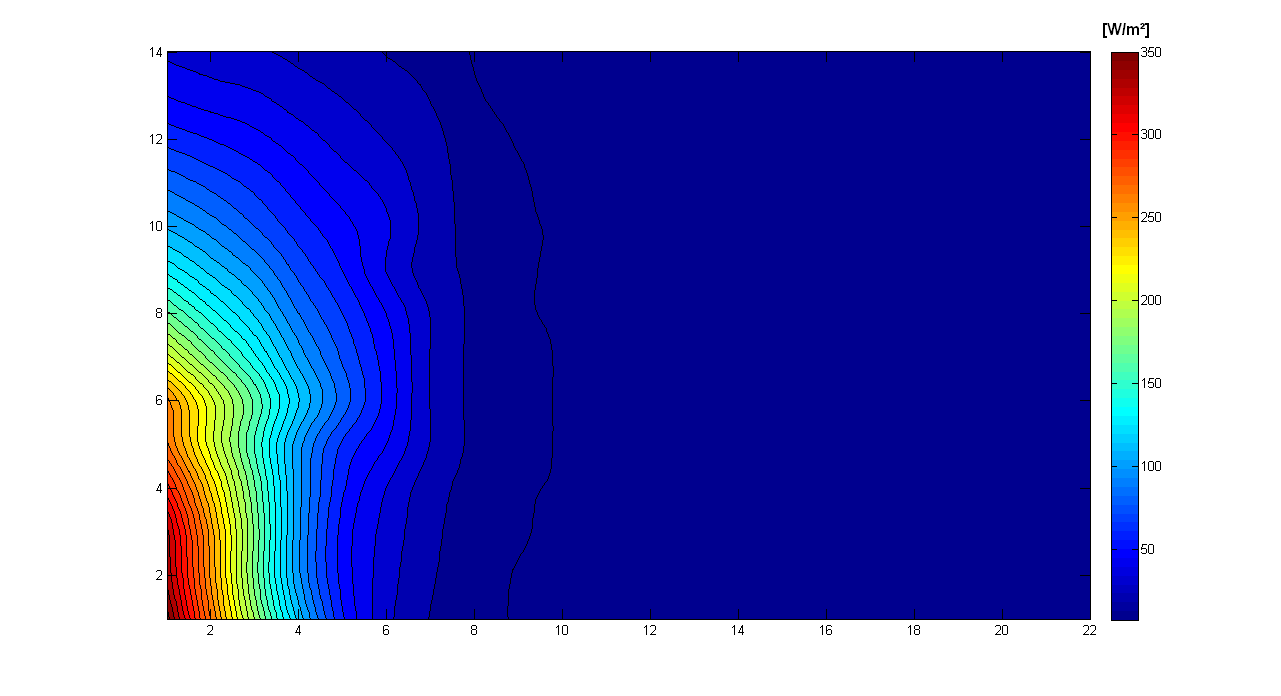
\includegraphics[width=0.49\textwidth]{img/E6a.png}}
\caption{Lampe E6}
\end{figure} 

\begin{figure}
    \subfigure[3D Ansicht]{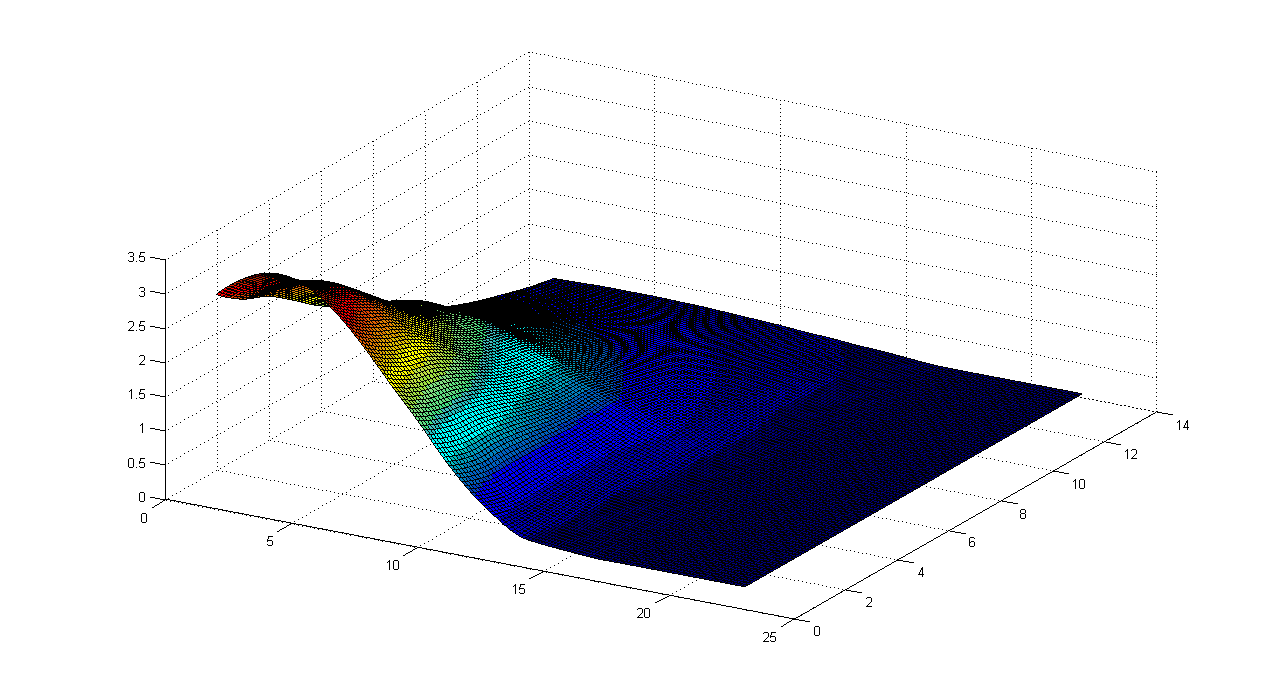
\includegraphics[width=0.49\textwidth]{img/E7.png}}
    \subfigure[Landkarte]{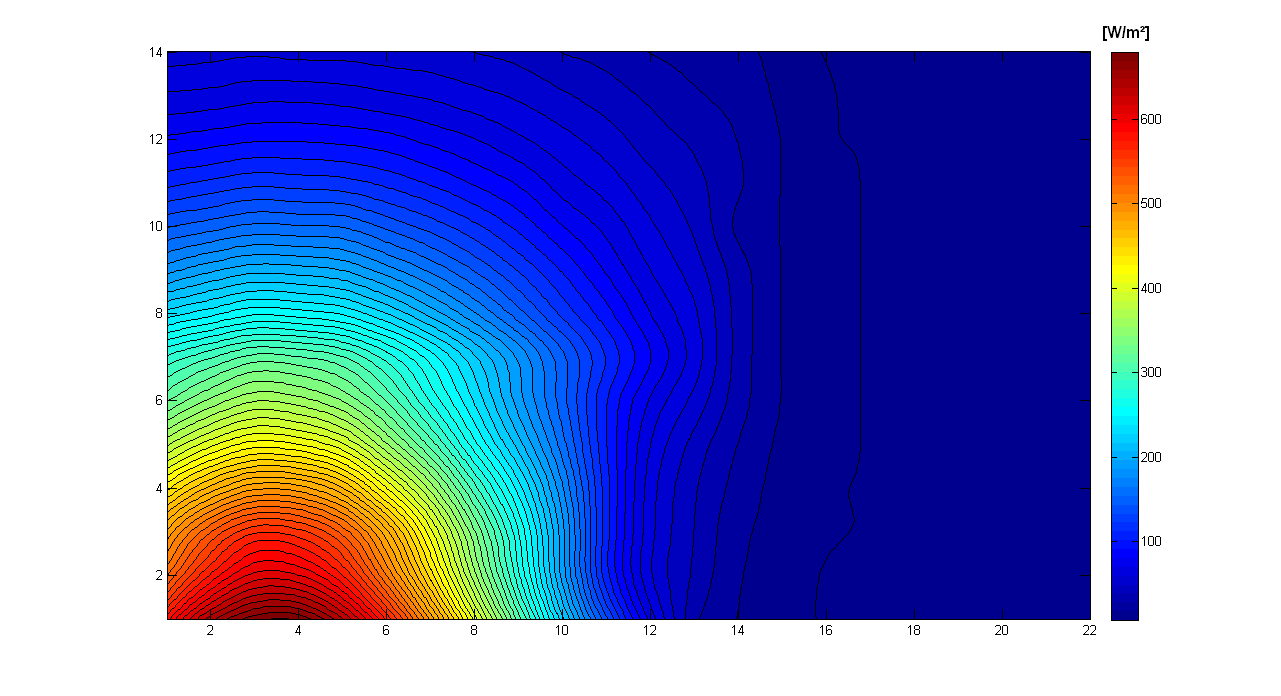
\includegraphics[width=0.49\textwidth]{img/E7a.png}}
\caption{Lampe E7}
\end{figure} 

\begin{figure}
    \subfigure[3D Ansicht]{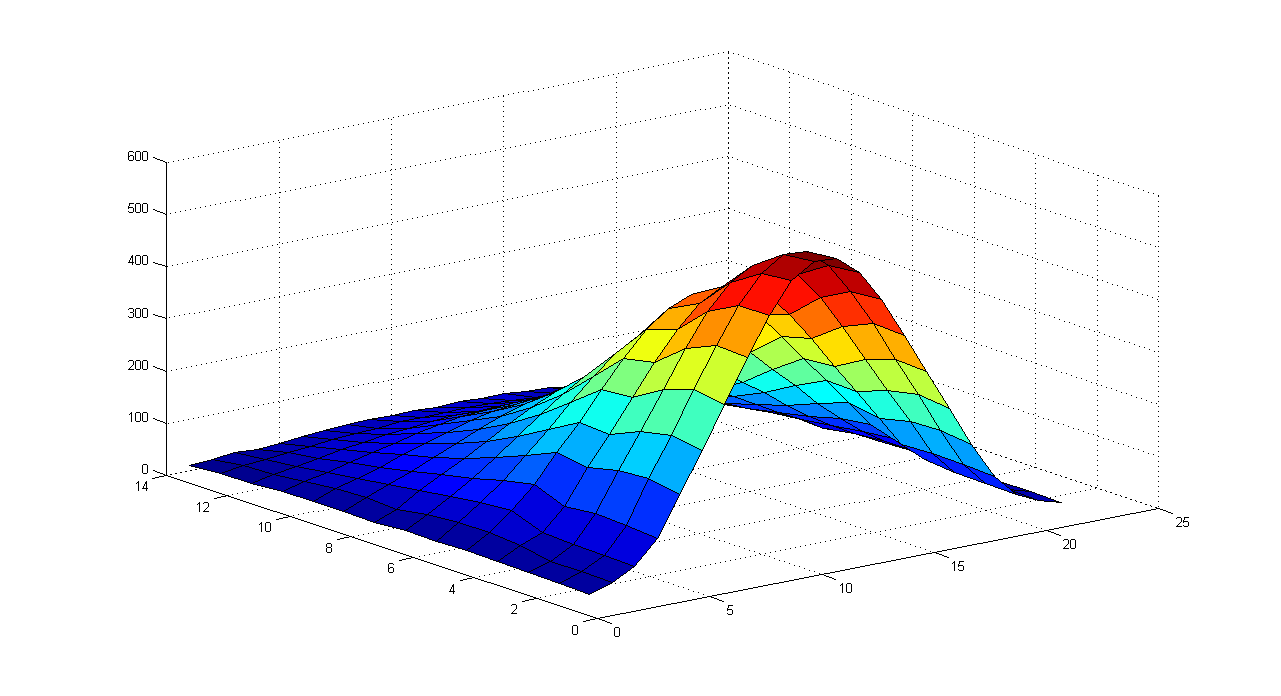
\includegraphics[width=0.49\textwidth]{img/E8.png}}
    \subfigure[Landkarte]{\includegraphics[width=0.49\textwidth]{img/E8a.png}}
\caption{Lampe E8}
\end{figure} 

\begin{figure}
    \subfigure[3D Ansicht]{\includegraphics[width=0.49\textwidth]{img/E9.png}}
    \subfigure[Landkarte]{\includegraphics[width=0.49\textwidth]{img/E9a.png}}
\caption{Lampe E9}
\end{figure} 

\begin{figure}
    \subfigure[3D Ansicht]{\includegraphics[width=0.49\textwidth]{img/E10.png}}
    \subfigure[Landkarte]{\includegraphics[width=0.49\textwidth]{img/E10a.png}}
\caption{Lampe E10}
\end{figure} 





 





\section{Schlussfolgerung}\thispagestyle{empty}

Der Roboter erleichtert die Messung der Bestrahlungsstärkemessung enorm.  




% Literaturverzeichnis
% Das Literaturverzeichnis kann auch nach einem allf"alligen Anhang positiioniert werden (siehe "`Leitfaden f"ur Bachelor- und Diplomarbeiten"', Version 2.0, Abschnitt 2.9).

% M"oglichkeit 1: Erzeugung des Literaturverzeichnisses mit BibTeX:
% Die Quellen sind in der Datei *.bib (hier Literatur.bib) einzugeben. Danach muss diese Vorlage einmal geTeXt werden, dann BibTeX angewendet werden und 
% anschliessend nochmals zweimal geTeXt werden.
% Im Text erfolgt die Zitierung mit dem Anker-Schl"usselwort, z.B. \cite{kop05}.
\bibliographystyle{IEEEtran}
\bibliography{Literatur}

% M"oglichkeit 2: Erzeugung eines Literaturverzeichnisses ohne BibTeX:
%\begin{thebibliography}{99}
%\bibitem[kop05]{kop05}
%H.~Kopka, {\em LaTeX, Band 1: Einf"uhrung}, Pearson Studium, M"unchen, 3.~Auflage, 2005.
%\bibitem[knu98]{knu98}
%F.~Mittelbach, M.~Goossens, J.~Braams, D.~Carlisle, and Ch. Rowley, {\em The LaTeX Companion}, 
%Addison-Wesley, 2nd edition, 2004.
%\end{thebibliography}

% Abbildungsverzeichnis
\listoffigures
\addcontentsline{toc}{chapter}{Abbildungsverzeichnis} % f"ugt den Eintrag "Abbildungsverzeichnis" im Inhaltsverzeichnis hinzu
\newpage

% Tabellenverzeichnis
\listoftables 
\addcontentsline{toc}{chapter}{Tabellenverzeichnis} % f"ugt den Eintrag "Tabellenverzeichnis" im Inhaltsverzeichnis hinzu
\newpage

% Abk"urzungsverzeichnis
% Bei Verwendung der Dokumentklasse "scrartcl" ist der Befehlt \addchap{Abk"urzungsverzeichnis} durch 
% \addsec{Abk"urzungsverzeichnis} zu ersetzen
\addchap{Abk"urzungsverzeichnis}
\hspace{-17mm}\begin{tabular}{>{\raggedleft}p{0.2\linewidth} p{0.75\linewidth} p{0.1\linewidth}}
www & World Wide Web \\
URL & Uniform Resource Locator
\end{tabular}


% Anh"ange
\begin{appendix}
\chapter{Sourcecode Arduino}

\begin{verbatim}
/*
Programm zum Steuern des Sonnensimulatormessroboters
 Version 1.0 
 */

#include <SD.h>

void vor(int sped);
void zuruck(int sped);
void left(int sped);
void right(int sped);
void tl(int sped);
void tr(int sped);
void ztl();
void ztr();
void vtl();
void vtr();
void halt(); 

// ADCs zum Auslesen der 3x3 Matrix
const int analogInPin0 = A9;  
const int analogInPin1 = A2;
const int analogInPin2 = A5;
const int analogInPin3 = A8;
const int analogInPin4 = A1;
const int analogInPin5 = A4;
const int analogInPin6 = A7;
const int analogInPin7 = A0;
const int analogInPin8 = A3;
const int analogInPin9 = A6;

// Ausgang zum Schalten der Infrarot-Leds
const int analogInPin10 = A10;

// ADC für Messwerte
const int analogInPin12 = A12;
const int analogInPin13 = A13;
const int analogInPin14 = A14;
const int analogInPin15 = A15;

// Digitalausg"ange zum Ansteuern der Motoren
int IN1M1 = 2;
int IN2M1 = 3;
int IN1M2 = 4;
int IN2M2 = 5;
int IN1M3 = 6;
int IN2M3 = 9;
int IN1M4 = 7;
int IN2M4 = 8;

// Sensorwerte der optischen Sensoren (beleuchtet)
int sensorValue0 = 0;        // value read from the pot
int sensorValue1 = 0;        // value read from the pot
int sensorValue2 = 0;        // value read from the pot
int sensorValue3 = 0;        // value read from the pot
int sensorValue4 = 0;        // value read from the pot
int sensorValue5 = 0;        // value read from the pot
int sensorValue6 = 0;        // value read from the pot
int sensorValue7 = 0;        // value read from the pot
int sensorValue8 = 0;        // value read from the pot
int sensorValue9 = 0;        // value read from the pot

// Sensorwerte der optischen Sensoren (unbeleuchtet)
int sensorValue0d = 0;        // value read from the pot
int sensorValue1d = 0;        // value read from the pot
int sensorValue2d = 0;        // value read from the pot
int sensorValue3d = 0;        // value read from the pot
int sensorValue4d = 0;        // value read from the pot
int sensorValue5d = 0;        // value read from the pot
int sensorValue6d = 0;        // value read from the pot
int sensorValue7d = 0;        // value read from the pot
int sensorValue8d = 0;        // value read from the pot
int sensorValue9d = 0;        // value read from the pot

// für Auswertung der opischen Sensoren
int A = 0;
int B = 0;
int C = 0;
int D = 0;
int E = 0;
int F = 0;
int G = 0;
int H = 0;
int I = 0;
int S = 0;

// Grenzwerte für hell (=white) und dunkel (=bleak)
int white = 400;
int white2 = 250;
int bleak = 100;
int bleak2 = 150;

// zur Berechnung der Lage der LInie
float x1,x2,x3,d,k;
float y1,y2,y3,d2,k2;

// einige Hilfsvariablen
char mode='s';
char richtung='v';
int _stop=0;
int vor_ein=0;
int zuruck_ein=0;

// für die Auswertung der Messwerte
long int  temp_modul = 0; 
long int temp_i=0;
long int _Isc = 0; 
long int time = 0; 

// zur Schreiben auf die SD Karte
const int chipSelect = 53;

// Z"ahlvariable für Messpunkt, Spalte und Reihe
int count = 0;
int count2 = 0;
int row = 1;

// zur Schreiben auf die SD Karte
String dataString = "";

// notwendig für die Kommunikation mit SD Karte
void setup() {
  pinMode(A10, OUTPUT);
  pinMode(53, OUTPUT);
  SD.begin(chipSelect);
}

// Definiert alle möglichen Bewegungen
void zuruck(int sped)  
{
  analogWrite(IN1M1,0);
  analogWrite(IN2M1,sped);   
  analogWrite(IN1M2,0);
  analogWrite(IN2M2,sped); 
  analogWrite(IN1M3,0);
  analogWrite(IN2M3,sped); 
  analogWrite(IN1M4,0);
  analogWrite(IN2M4,sped);
}  

void vor(int sped)  
{
  analogWrite(IN1M1,sped);
  analogWrite(IN2M1,0);   
  analogWrite(IN1M2,sped);
  analogWrite(IN2M2,0); 
  analogWrite(IN1M3,sped);
  analogWrite(IN2M3,0); 
  analogWrite(IN1M4,sped);
  analogWrite(IN2M4,0);
}

void left(int sped)  
{
  analogWrite(IN1M1,0);
  analogWrite(IN2M1,sped);   
  analogWrite(IN1M2,sped);
  analogWrite(IN2M2,0); 
  analogWrite(IN1M3,sped);
  analogWrite(IN2M3,0); 
  analogWrite(IN1M4,0);
  analogWrite(IN2M4,sped);
}

void right(int sped)  
{
  analogWrite(IN1M1,sped);
  analogWrite(IN2M1,0);   
  analogWrite(IN1M2,0);
  analogWrite(IN2M2,sped); 
  analogWrite(IN1M3,0);
  analogWrite(IN2M3,sped); 
  analogWrite(IN1M4,sped);
  analogWrite(IN2M4,0);
}

void tr(int sped)
{
  analogWrite(IN1M1,sped);
  analogWrite(IN2M1,0);   
  analogWrite(IN1M2,0);
  analogWrite(IN2M2,sped); 
  analogWrite(IN1M3,sped);
  analogWrite(IN2M3,0); 
  analogWrite(IN1M4,0);
  analogWrite(IN2M4,sped);
}

void tl(int sped)
{
  analogWrite(IN1M1,0);
  analogWrite(IN2M1,sped);   
  analogWrite(IN1M2,sped);
  analogWrite(IN2M2,0); 
  analogWrite(IN1M3,0);
  analogWrite(IN2M3,sped); 
  analogWrite(IN1M4,sped);
  analogWrite(IN2M4,0);
}

void vtr()
{   
  analogWrite(IN1M1,64);
  analogWrite(IN2M1,0);   
  analogWrite(IN1M2,0);
  analogWrite(IN2M2,64); 
  analogWrite(IN1M3,128);
  analogWrite(IN2M3,0); 
  analogWrite(IN1M4,128);
  analogWrite(IN2M4,0);
}

void vtl()
{   
  analogWrite(IN1M1,0);
  analogWrite(IN2M1,64);   
  analogWrite(IN1M2,64);
  analogWrite(IN2M2,0); 
  analogWrite(IN1M3,128);
  analogWrite(IN2M3,0); 
  analogWrite(IN1M4,128);
  analogWrite(IN2M4,0);
}

void ztr()  
{
  analogWrite(IN1M1,0);
  analogWrite(IN2M1,64);   
  analogWrite(IN1M2,0);
  analogWrite(IN2M2,64); 
  analogWrite(IN1M3,0);
  analogWrite(IN2M3,64); 
  analogWrite(IN1M4,64);
  analogWrite(IN2M4,0);
}  

void ztl()  
{
  analogWrite(IN1M1,0);
  analogWrite(IN2M1,64);   
  analogWrite(IN1M2,0);
  analogWrite(IN2M2,64); 
  analogWrite(IN1M3,64);
  analogWrite(IN2M3,0); 
  analogWrite(IN1M4,0);
  analogWrite(IN2M4,64);
}  

void halt()  
{
  analogWrite(IN1M1,0);
  analogWrite(IN2M1,0);   
  analogWrite(IN1M2,0);
  analogWrite(IN2M2,0); 
  analogWrite(IN1M3,0);
  analogWrite(IN2M3,0); 
  analogWrite(IN1M4,0);
  analogWrite(IN2M4,0);
}


// Hauptschleife
void loop() 
{

  // Werte ohne Beleuchtung:
  sensorValue0d = analogRead(analogInPin0);   
  sensorValue1d = analogRead(analogInPin1);  
  sensorValue2d = analogRead(analogInPin2);  
  sensorValue3d = analogRead(analogInPin3);  
  sensorValue4d = analogRead(analogInPin4);  
  sensorValue5d = analogRead(analogInPin5);  
  sensorValue6d = analogRead(analogInPin6);  
  sensorValue7d = analogRead(analogInPin7);  
  sensorValue8d = analogRead(analogInPin8);  
  sensorValue9d = analogRead(analogInPin9);  
  digitalWrite(A10, HIGH);  // LED ein
  delay(2); 
  // Werte mit Beleuchtung:
  sensorValue0 = analogRead(analogInPin0);   
  sensorValue1 = analogRead(analogInPin1);  
  sensorValue2 = analogRead(analogInPin2);  
  sensorValue3 = analogRead(analogInPin3);  
  sensorValue4 = analogRead(analogInPin4);  
  sensorValue5 = analogRead(analogInPin5);  
  sensorValue6 = analogRead(analogInPin6);  
  sensorValue7 = analogRead(analogInPin7);  
  sensorValue8 = analogRead(analogInPin8);  
  sensorValue9 = analogRead(analogInPin9);  
  digitalWrite(A10, LOW);

  A = sensorValue1 - sensorValue1d;
  B = sensorValue2 - sensorValue2d;
  C = sensorValue3 - sensorValue3d;
  D = sensorValue4 - sensorValue4d;
  E = sensorValue5 - sensorValue5d;
  F = sensorValue6 - sensorValue6d;
  G = sensorValue7 - sensorValue7d;
  H = sensorValue8 - sensorValue8d;
  I = sensorValue9 - sensorValue9d;

  S = sensorValue0 - sensorValue0d;

  // zum Erkennen der Linie bei vor- oder zurückfahren 
  x1 = ((C-A)/float(2*A-4*B+2*C));
  x2 = ((F-D)/float(2*D-4*E+2*F));
  x3 = ((I-G)/float(2*G-4*H+2*I));

  d = (x1 + x2 + x3)/3.; // ~ Abstand von der Ideallinie
  k = (x1-x3)/2.;  // Steigung = Verdrehung

  // zum Erkennen der Linie bei links- oder rechtsfahren
  y1 = ((G-A)/float(2*A-4*D+2*G));
  y2 = ((H-B)/float(2*B-4*E+2*H));
  y3 = ((I-C)/float(2*C-4*F+2*I));

  d2 = (y1+y2+y3)/3.;
  k2 = (y3-y1)/2.;

  if( S < bleak2) _stop=0;

  halt();

  if(E>bleak2)
  {

    switch(mode)
    {
    case 's':     // Start
      { 
        halt();
        delay(60000);  // 1 Minuten warten
        mode='v';
      }
      break;

      // Messmode
    case 'e':   // Ende
      {
        halt();
      }
      break;

    case 'm':   // Messen
      { 
        count = count + 1;  // Anzahl der Haltepunkte
        count2 = count2 + 1; 
        dataString = "";
        _stop=1;
        halt();

        delay(250);   // damit die Str"ome der Fahrmotoren keinen Einfluss auf die AD-Wandlung haben

        _Isc = 0;
        temp_modul = 0;
        temp_i = 0;

        // Mittelung über jeweils 500 Messwerte
        for(int i = 0; i < 500 ; i++)
        {
          _Isc = _Isc + analogRead(analogInPin13);  
          temp_modul = temp_modul + analogRead(analogInPin12); 
          temp_i =  temp_i + analogRead(analogInPin15); 
        }
        _Isc = int(_Isc/500.0);
        temp_modul = int(temp_modul/500.0);
        temp_i = int(temp_i/500.0);
        time = millis();

        // Schreiben aud SD-Karte
        dataString += String(time);
        dataString += "\t"; 
        dataString += String(_Isc); 
        dataString += "\t"; 
        dataString += String(temp_modul); 
        dataString += "\t"; 
        dataString += String(temp_i); 
        dataString += "\t"; 
        dataString += String(count); 
        dataString += "\t"; 
        dataString += String(count2); 
        dataString += "\t"; 
        dataString += String(row); 

        // Schreibe aud SD Card
        File dataFile = SD.open("datalog.txt", FILE_WRITE);
        if (dataFile) {
          dataFile.println(dataString);
          dataFile.close();
        }

        // zurück in den Bewegungsmode
        if(richtung=='v') mode='v';
        if(richtung=='z') mode='z';

      }
      break;

    case 'v':   // Vorwärtsfahren
      { 

        richtung='v';

        if(d>0.02)  vtr();
        else 
        {  
          if(d>-0.02)  vor(128);
          else 
            vtl();
        }

        //if((C<bleak)&&(A<bleak))
        if(A<bleak2)
        {
          if(k>0.01) tr(64);
          else
          {
            if(k<-0.01) tl(64);
          }

          if(d>0.025) right(64);
          else
          {
            if(d<-0.025) left(64);
          }
        }   
        if((A>white)&&(B>white)) mode='a'; 

        if((_stop==0)&&(S>white2)) mode='m';   


      }
      break;

    case 'z': // Rückwärtsfahren
      { 

        richtung='z';

        if(d>0.02)  ztr();
        else 
        {  
          if(d>-0.02)  zuruck(128);
          else  ztl();
        }

        //if((G<bleak)&&(I<bleak))
        if(G<bleak2)
        {
          if(k>0.01) tr(64);
          else
          {
            if(k<-0.01) tl(64);
          }

          if(d>0.025) right(64);
          else
          {
            if(d<-0.025) left(64);
          }
        }
        if((G>white)&&(H>white)) mode='c';

        if((_stop==0)&&(S>white2)) mode='m';  

        if((I<bleak)&&(H<bleak)&&(G<bleak)) mode='e';

      }
      break; 

    case 'r':     //nach rechts
      {
        richtung='r';
        count2 = 0;

        right(128);
        if(D>white2)
        {
          if(d2>0.04) vor_ein=1;
          if(d2<0.02) vor_ein=0;
          if(d2<-0.04) zuruck_ein=1;
          if(d2>-0.02) zuruck_ein=0;

          if(vor_ein==1) vor(64);
          if(zuruck_ein==1) zuruck(64);

          if((vor_ein==0)&&(zuruck_ein==0))
          {
            if(k2>0.02) tr(64);
            else
            {
              if(k2<-0.02) tl(64);
            }
          }
        }

        if((D<bleak)&&(G<bleak)&&(A<bleak)) 
        { 
          mode='b';
        }

      } 
      break;

    case 'l':    // auch nach rechts 
      {
        richtung=='l';
        count2 = 0;

        right(128);
        //if((C<bleak)&&(I<bleak))
        if(D>white2)
        {
          if(d2>0.04) vor_ein=1;
          if(d2<0.02) vor_ein=0;
          if(d2<-0.04) zuruck_ein=1;
          if(d2>-0.02) zuruck_ein=0;

          if(vor_ein==1) vor(64);
          if(zuruck_ein==1) zuruck(64);

          if((vor_ein==0)&&(zuruck_ein==0))
          {
            if(k2>0.02) tr(64);
            else
            {
              if(k2<-0.02) tl(64);
            }
          }
        }

        if((D<bleak)&&(G<bleak)&&(A<bleak))
        { 
          mode='d';
        }

      } 
      break;

    case 'a':  // Um die Ecke fahren
      {
        if((A>bleak2)&&(B>bleak2)) vor(64);
        else 
        { 
          right(64);
          delay(700);
          halt();
          row = row +1 ;

          mode='r';

        }
      } 
      break; 

    case 'b':  // Um die Ecke fahren
      {

        zuruck(64);
        delay(850);
        halt();
        delay(500);

        mode='x';

      } 
      break; 

    case 'x':
      {
        if(d>0.025) right(64);

        if(d<-0.025) left(64);

        if((d<0.1)&&(d>-0.1)) mode='y';
      }
      break;

    case 'y':
      {
        if(k>0.01) tr(32);

        if(k<-0.01) tl(32);

        if((k<0.04)&&(k>-0.04)) mode='z';
      }
      break;

    case 'c':  // Um die Ecke fahren
      {
        if((H>bleak2)&&(G>bleak2 )) zuruck(64);
        else 
        { 
          right(64);
          delay(700);
          halt();
          row = row +1 ;

          mode='l';
        }
      } 
      break; 

    case 'd':  // Um die Ecke fahren
      {

        vor(64);
        delay(850);
        halt();
        delay(500);
        mode='q';

      } 
      break; 

    case 'q':
      {
        if(d>0.025) right(64);

        if(d<-0.025) left(64);

        if((d<0.1)&&(d>-0.1))       mode='p';
      }
      break;


    case 'p':
      {
        if(k>0.01) tr(32);

        if(k<-0.01) tl(32);

        if((k<0.04)&&(k>-0.04)) mode='v'; 

      }
      break;
    } 
  }   


  else 
  {  
    if((richtung=='v')||(richtung=='z'))
    {
      if((A>bleak2)||(D>bleak2)||(G>bleak2)||(C>bleak2)||(F>bleak2)||(I>bleak2))
      {
        if((A+D+G)>(C+F+I)) right(128);
        else left(128);
      }
      else halt();
    }


    if((richtung=='r')||(richtung=='l'))
    {
      if((A>bleak2)||(B>bleak2)||(C>bleak2)||(G>bleak2)||(H>bleak2)||(I>bleak2))
      {
        if((A+B+C)>(G+H+I)) vor(64);
        else zuruck(64);
      }
      else halt();
    }
  }

  delay(5); 

}
\end{verbatim}

\chapter{Sourcecode Auswertung}



\begin{verbatim}

% Graphische Auswertung der Robotermesswerte

close all;
clc;
clear all;

% "Offnen der Datei, welche eine Messfahrt mit genau 308 Messwerten
% enthalten muss
fid = fopen('data1.txt', 'r');
a = fscanf(fid, '%g %g', [7 308])     
a = a';
fclose(fid)

j=1; k=1; l=1;

% Umwandeln der 1 dimensionalen Modultemperatur ADC-Werte in eine Matrix:
for(i=0:307)
    if(mod(i,28)>13) k = 28- mod(i,28);
    else k = mod(i,14)+1;
    end
    Tm(k,l)=a(i+1,3);
    if(mod(i+1,14)==0) l=l+1;
    end
end

% Umrechnung der ADC-Werte in Temeratur:
Rm = (Tm +4038.9)/40.107;  % ADC --> Widerstand
TTm = (Rm-100.03)/0.3879;  % Widerstand --> Temperatur

j=1; k=1; l=1;

% Umwandeln der 1 dimensionalen Innentemperatur ADC-Werte in eine Matrix:
for(i=0:307)
    if(mod(i,28)>13) k = 28- mod(i,28);
    else k = mod(i,14)+1;
    end
    Ti(k,l)=a(i+1,4);
    if(mod(i+1,14)==0) l=l+1;
    end
end

% Umrechnung der ADC-Werte in Temeratur:
Ri = (Ti +4023.6)/40.027;  % ADC --> Widerstand
TTi = (Ri-100.03)/0.3879;  % Widerstand --> Temperatur

j=1; k=1; l=1;

% Umwandeln der 1 dimensionalen Kurzschlusstrom ADC-Werte in eine Matrix:
for(i=0:307)
    if(mod(i,28)>13) k = 28- mod(i,28);
    else k = mod(i,14)+1;
    end
    I(k,l)=a(i+1,2);
    if(mod(i+1,14)==0) l=l+1;
    end
end

% Umrechnung der ADC-Werte in Ampere:

A = (I +4.5766)/119.2;   % ADC --> Ampere
A = A - (TTm-25)*0.004;  % Temperaturkorrektur



[XI,YI] = meshgrid(1:.125:22, 1:.125:14);

Ai = interp2(A,XI,YI,'cubic'); % Interpolation

A_max = max(max(Ai));
A_min = min(min(Ai));

Normiert = Ai / A_max * 1.1;

w = (A_max - A_min)/(A_max + A_min) * 100  % maximale Abweichung in Protzent

% Graphische Darstellung des Stromes
figure;
surf(XI,YI,Ai);   % in Ampere


% Graphische Darstellung des normierten Stromes
zlevs2 = 0.9:0.01:1.1;
figure;
[C,h] = contourf(XI,YI,Normiert,zlevs2);
set(h,'ShowText','on','TextStep',get(h,'LevelStep')*2)
colorbar;

% Graphische Darstellung der Modultemperatur
figure;
surf(TTm); 

% Graphische Darstellung der Umgebungstemperatur
figure;
surf(TTi);

\end{verbatim} 

\end{appendix}


\end{document}
